\chapter{RESULTS AND DISCUSSION}
This chapter describes the implementation and results of the empirical analysis
outlined above.  Each section of this chapter details one of the three main
tasks of the empirical analysis.  The first task is to create synthetic data,
the second to train the SOMs and finally to apply the diagnostics.

\section{Data}
To test out their Geodesic SOM, \cite{wu2006} generate a synthetic data set
consisting of seven clusters in three dimmensions.  Each cluster is normally distributed and has a
standard diviation of one.  The first cluster is centered at the orgin, the
others are ten units out each axis. 
%The data will be generated with the common technique of rejection sampling,
%where n high dimensional seeds are chosen at random, samples will be taken
%at random from a uniform distribution, if the sample falls with in radius r of
%any seed it is accepted, if it does not, single random number is drawn, if that
%number is \(<\) 0.05\% the sample is accepted as noise, else the sample is rejected.

\section{Training}
Before we can go on to addressing the research questions we need to train a
series of SOMs. One problem that we will face is a small group size when the
neurons of a given SOM are grouped by their degree.  For example in the rook
topology there are only four neurons that have a degree of two, the four
corners. The rest of the neurons have three or four neighbors depending on
whether they are on the edge or not. To deal with this problem we will try to
increase the sample size by combining the results of many SOMs trained with
similar data.

The four topologies are tested. These are the Rook, Hexagonal, Geodesic Sphere
and a forth topology based on a \cite{Rakhmanov94}. As mentioned before
\cite{Rakhmanov94} suggest a method for distributing an arbitrary number of
point on to the surface of a sphere.  Delaunay triangulation is applied to the
result of this method producing a topological structure for the points.  This
topology shall be is referred to simply as ``spherical.''  As shown in figure
\ref{fig:nSize} the achievable network size is rather limited in the geodesic
SOM.  An eight frequency geodesic sphere has 642 nodes. The hexagon and rook
topologies can achieve 644 nodes when the dimensions set to 28 by 23. The
spherical topology will be set to 642 nodes.

Ten synthetic datasets are generated using the parameters described in the
previous section. The datasets are used to train SOMs for each topology
resulting in another forty SOMs. The average internal variance of these SOMs
are summarized in Table \ref{ivtable3} and Table \ref{ivtable3:n}.  We find that the mean internal
variance seems to remain fairly stable, this suggests that we can combine the
results of each simulation within a given topology. In the rook topology we
will now have up to forty\footnote{We can only measure the internal variance
when a neuron captures two or more observations from the training data.
Therefore, it would be possible to have less than forty measurements.}
internal variance measurements for neurons with only two neighbors.

\begin{table}[hbt]
\centering
\caption{Mean IV for each simulation, by topology, 7clusters 3dims, no noise}
\label{ivtable3}
\begin{tabular}{|c||c|c|c|c|}
\hline
\textbf{Simulation Number} & Geodesic & Graph & Hex & Rook \\
\hline
\hline
\textbf{1} & 0.0277 & 0.0277 & 0.0285 & 0.0289 \\
\hline
\textbf{2} & 0.0281 & 0.0281 & 0.0291 & 0.0295 \\
\hline
\textbf{3} & 0.0278 & 0.0280 & 0.0286 & 0.0292 \\
\hline
\textbf{4} & 0.0280 & 0.0282 & 0.0286 & 0.0293 \\
\hline
\textbf{5} & 0.0279 & 0.0280 & 0.0289 & 0.0296 \\
\hline
\textbf{6} & 0.0278 & 0.0274 & 0.0285 & 0.0290 \\
\hline
\textbf{7} & 0.0286 & 0.0283 & 0.0294 & 0.0297 \\
\hline
\textbf{8} & 0.0284 & 0.0285 & 0.0294 & 0.0298 \\
\hline
\textbf{9} & 0.0283 & 0.0282 & 0.0293 & 0.0295 \\
\hline
\textbf{10} & 0.0285 & 0.0285 & 0.0293 & 0.0298 \\
\hline
\end{tabular} \end{table}


\begin{table}[hbt]
\centering
\caption{Mean IV for each simulation, by topology, 7clusters,3dims, layer of
noise}
\label{ivtable3:n}
\begin{tabular}{|c||c|c|c|c|}
\hline
\textbf{Simulation Number} & Geodesic & Graph & Hex & Rook \\
\hline
\hline
\textbf{1} & 0.0545 & 0.0539 & 0.0528 & 0.0525 \\
\hline
\textbf{2} & 0.0551 & 0.0551 & 0.0551 & 0.0550 \\
\hline
\textbf{3} & 0.0541 & 0.0543 & 0.0532 & 0.0527 \\
\hline
\textbf{4} & 0.0552 & 0.0554 & 0.0539 & 0.0543 \\
\hline
\textbf{5} & 0.0548 & 0.0544 & 0.0548 & 0.0527 \\
\hline
\textbf{6} & 0.0549 & 0.0540 & 0.0541 & 0.0548 \\
\hline
\textbf{7} & 0.0552 & 0.0547 & 0.0542 & 0.0545 \\
\hline
\textbf{8} & 0.0544 & 0.0548 & 0.0540 & 0.0534 \\
\hline
\textbf{9} & 0.0554 & 0.0551 & 0.0540 & 0.0533 \\
\hline
\textbf{10} & 0.0546 & 0.0552 & 0.0543 & 0.0542 \\
\hline
\end{tabular} \end{table}



\section{Diagnostics}
This section applies the our three diagnositcs to the SOMs that were trained
above.  All three build on the idea of an internal variance \(IV\). The
internal variance of neuron (\(i\)) is defined as,
 \begin{equation}
   {IV_i} = \frac{2}{{n_i}^2-{n_i}}\sum_{j=1}^{n_i}\sum_{k=j}^{n_i} ||{x_{ij}}-{x_{ik}}||
 \label{eqno1}
 \end{equation}
where, \(n_i\) is the number of observations mapped to \(i\), and \(x_i\) are
the input vectors mapped to \(i\).

The first diagnostic looks at how internal variance changes with a neuron's first
order neighborhood size, or degree.  The second compares the overall, or mean
internal variance accross topoliges.  The third visualizes the internal
variance of each SOM.

\subsection{Internal variance vs. first-order neighborhood size}
After the internal variance and degree of each neuron are calculated we
group the neurons for a given topology by their degree. The number for groups
we end up with varies by topology. Figure \ref{boxplot} offers a visualization
of these groups for each topology.  Each sub-figure shows a series of box
plots, each representing the distribution of internal variance within a given
group.  It was originally expected that the internal variances would be lower
for groups with larger degrees. This figure suggests that is only true for the
``flat'' topologies.

\begin{figure}[hbt]
\centering
\subfigure[Rook Topology]{
  \label{boxplot:rook}
  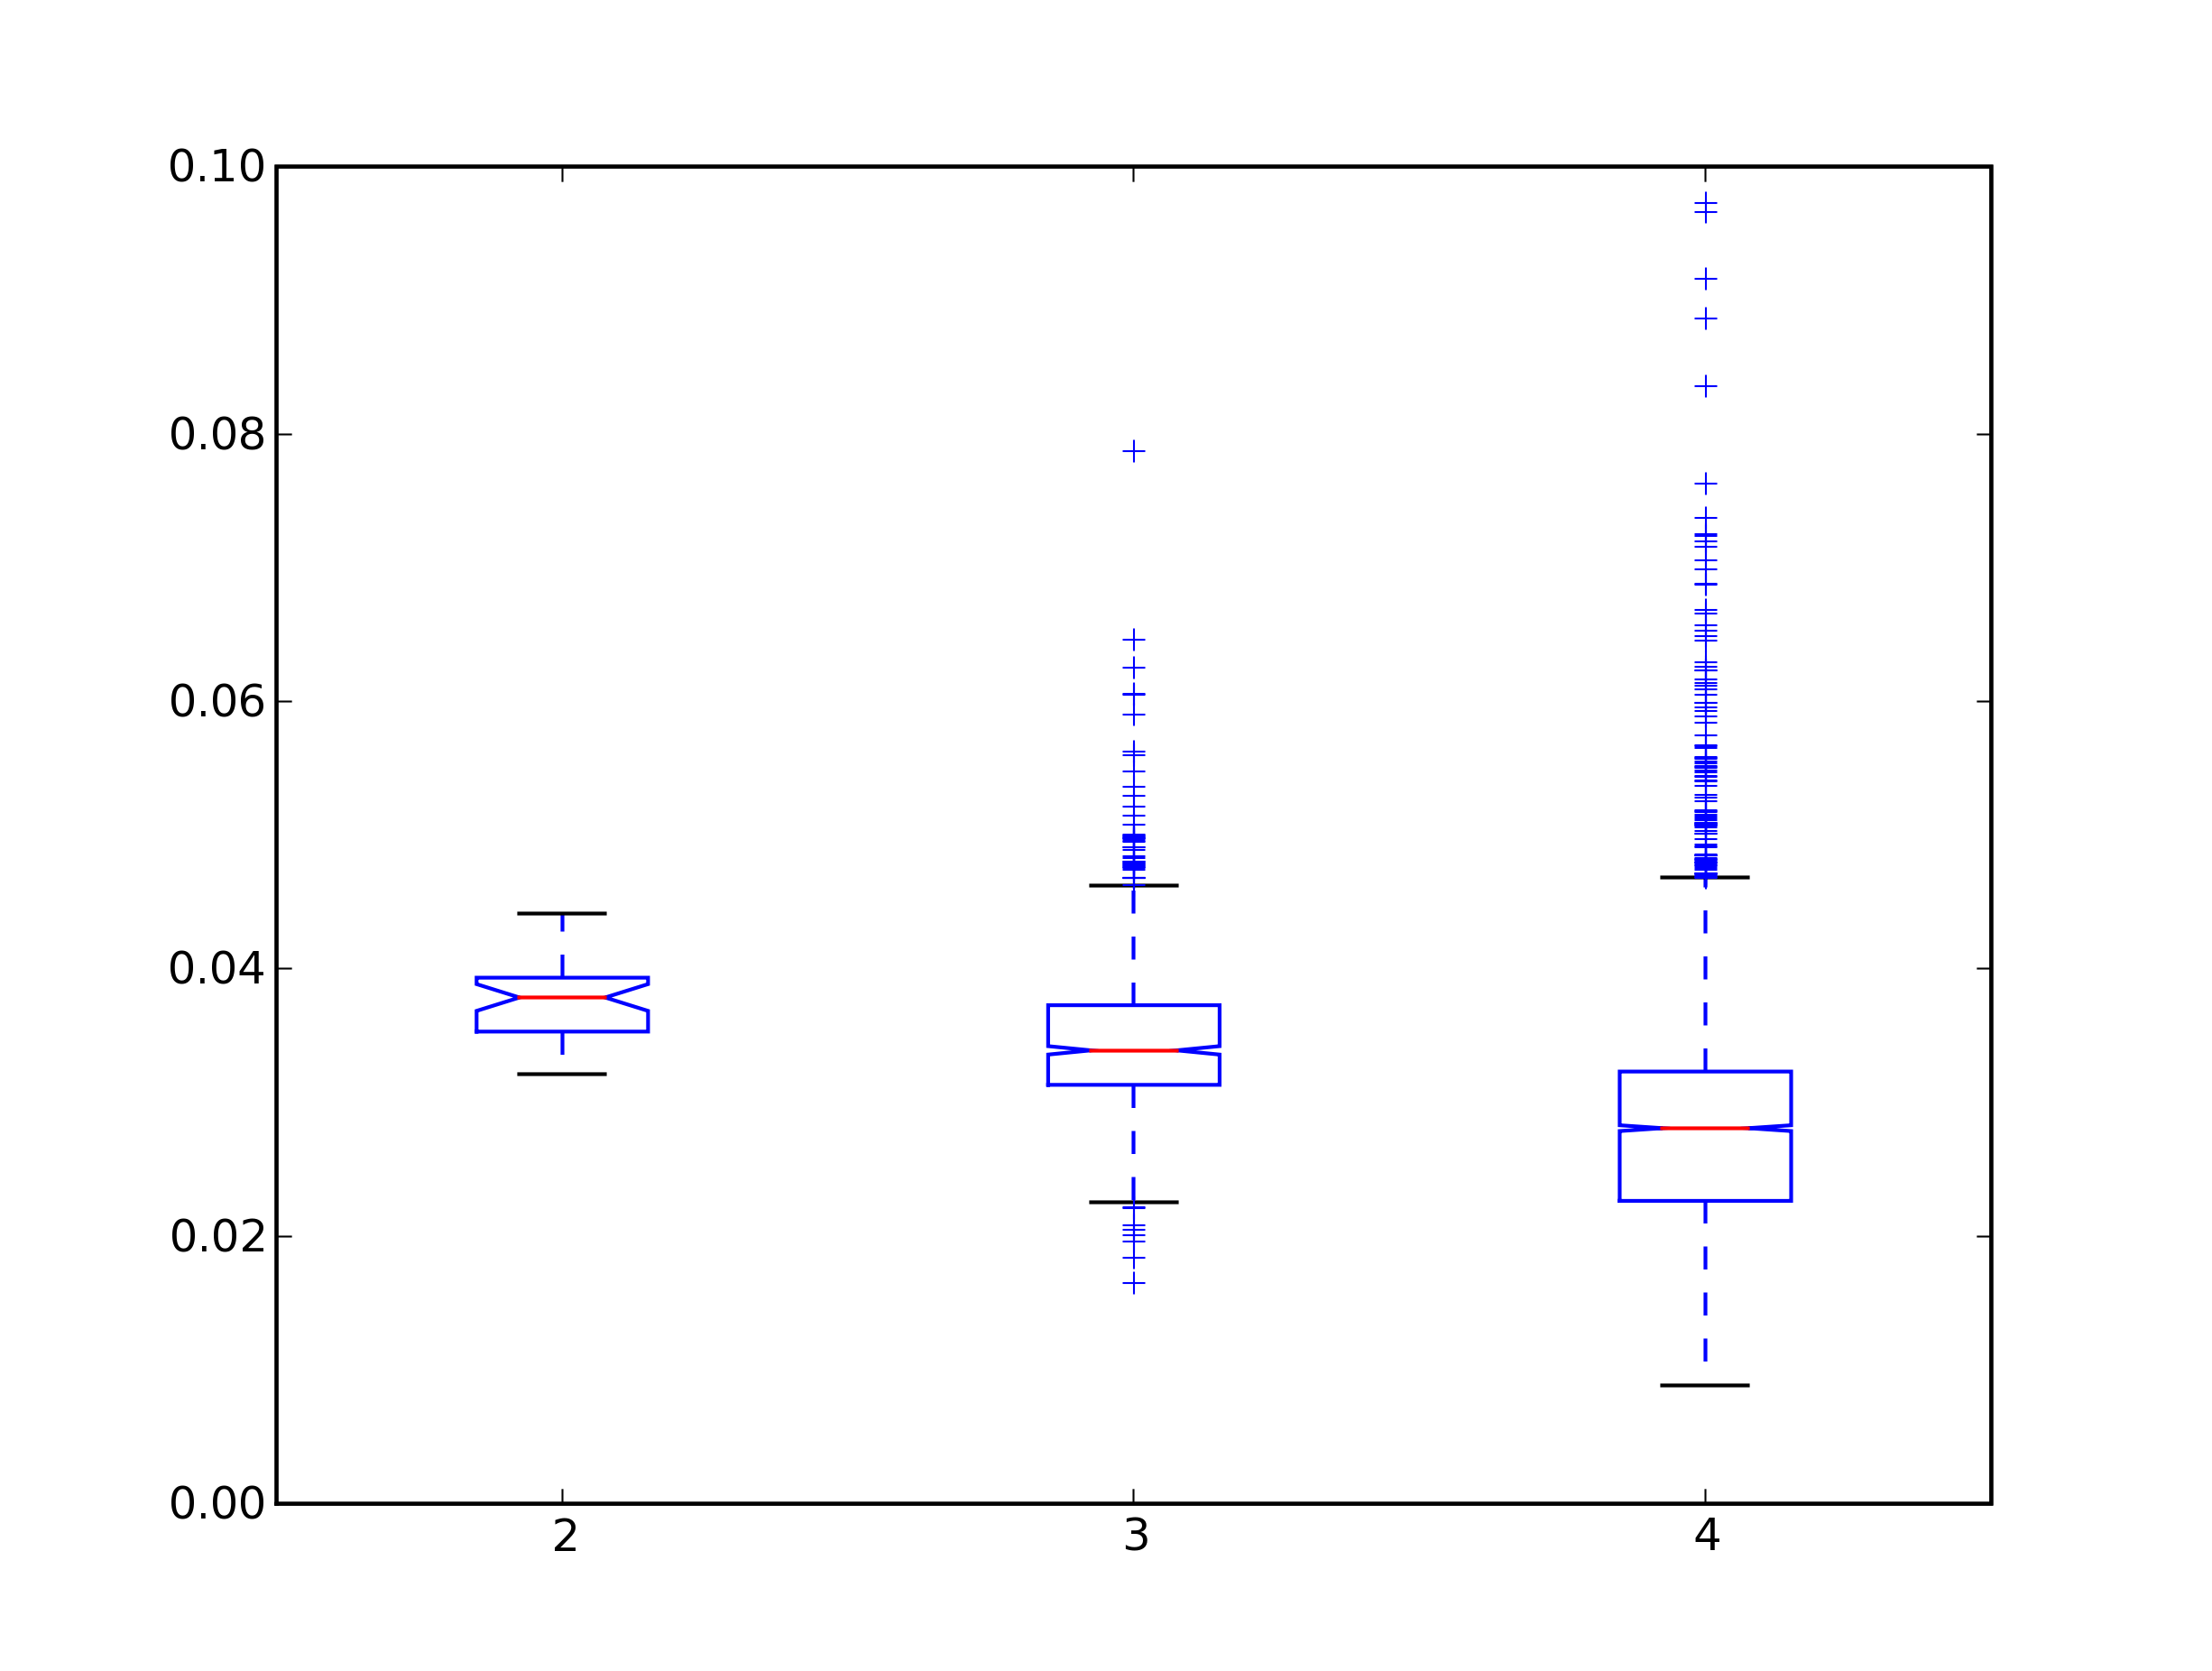
\includegraphics[width=.45\linewidth]{rook_iv_box.png}
}
\subfigure[Hexagonal Topology]{
  \label{boxplot:hex}
  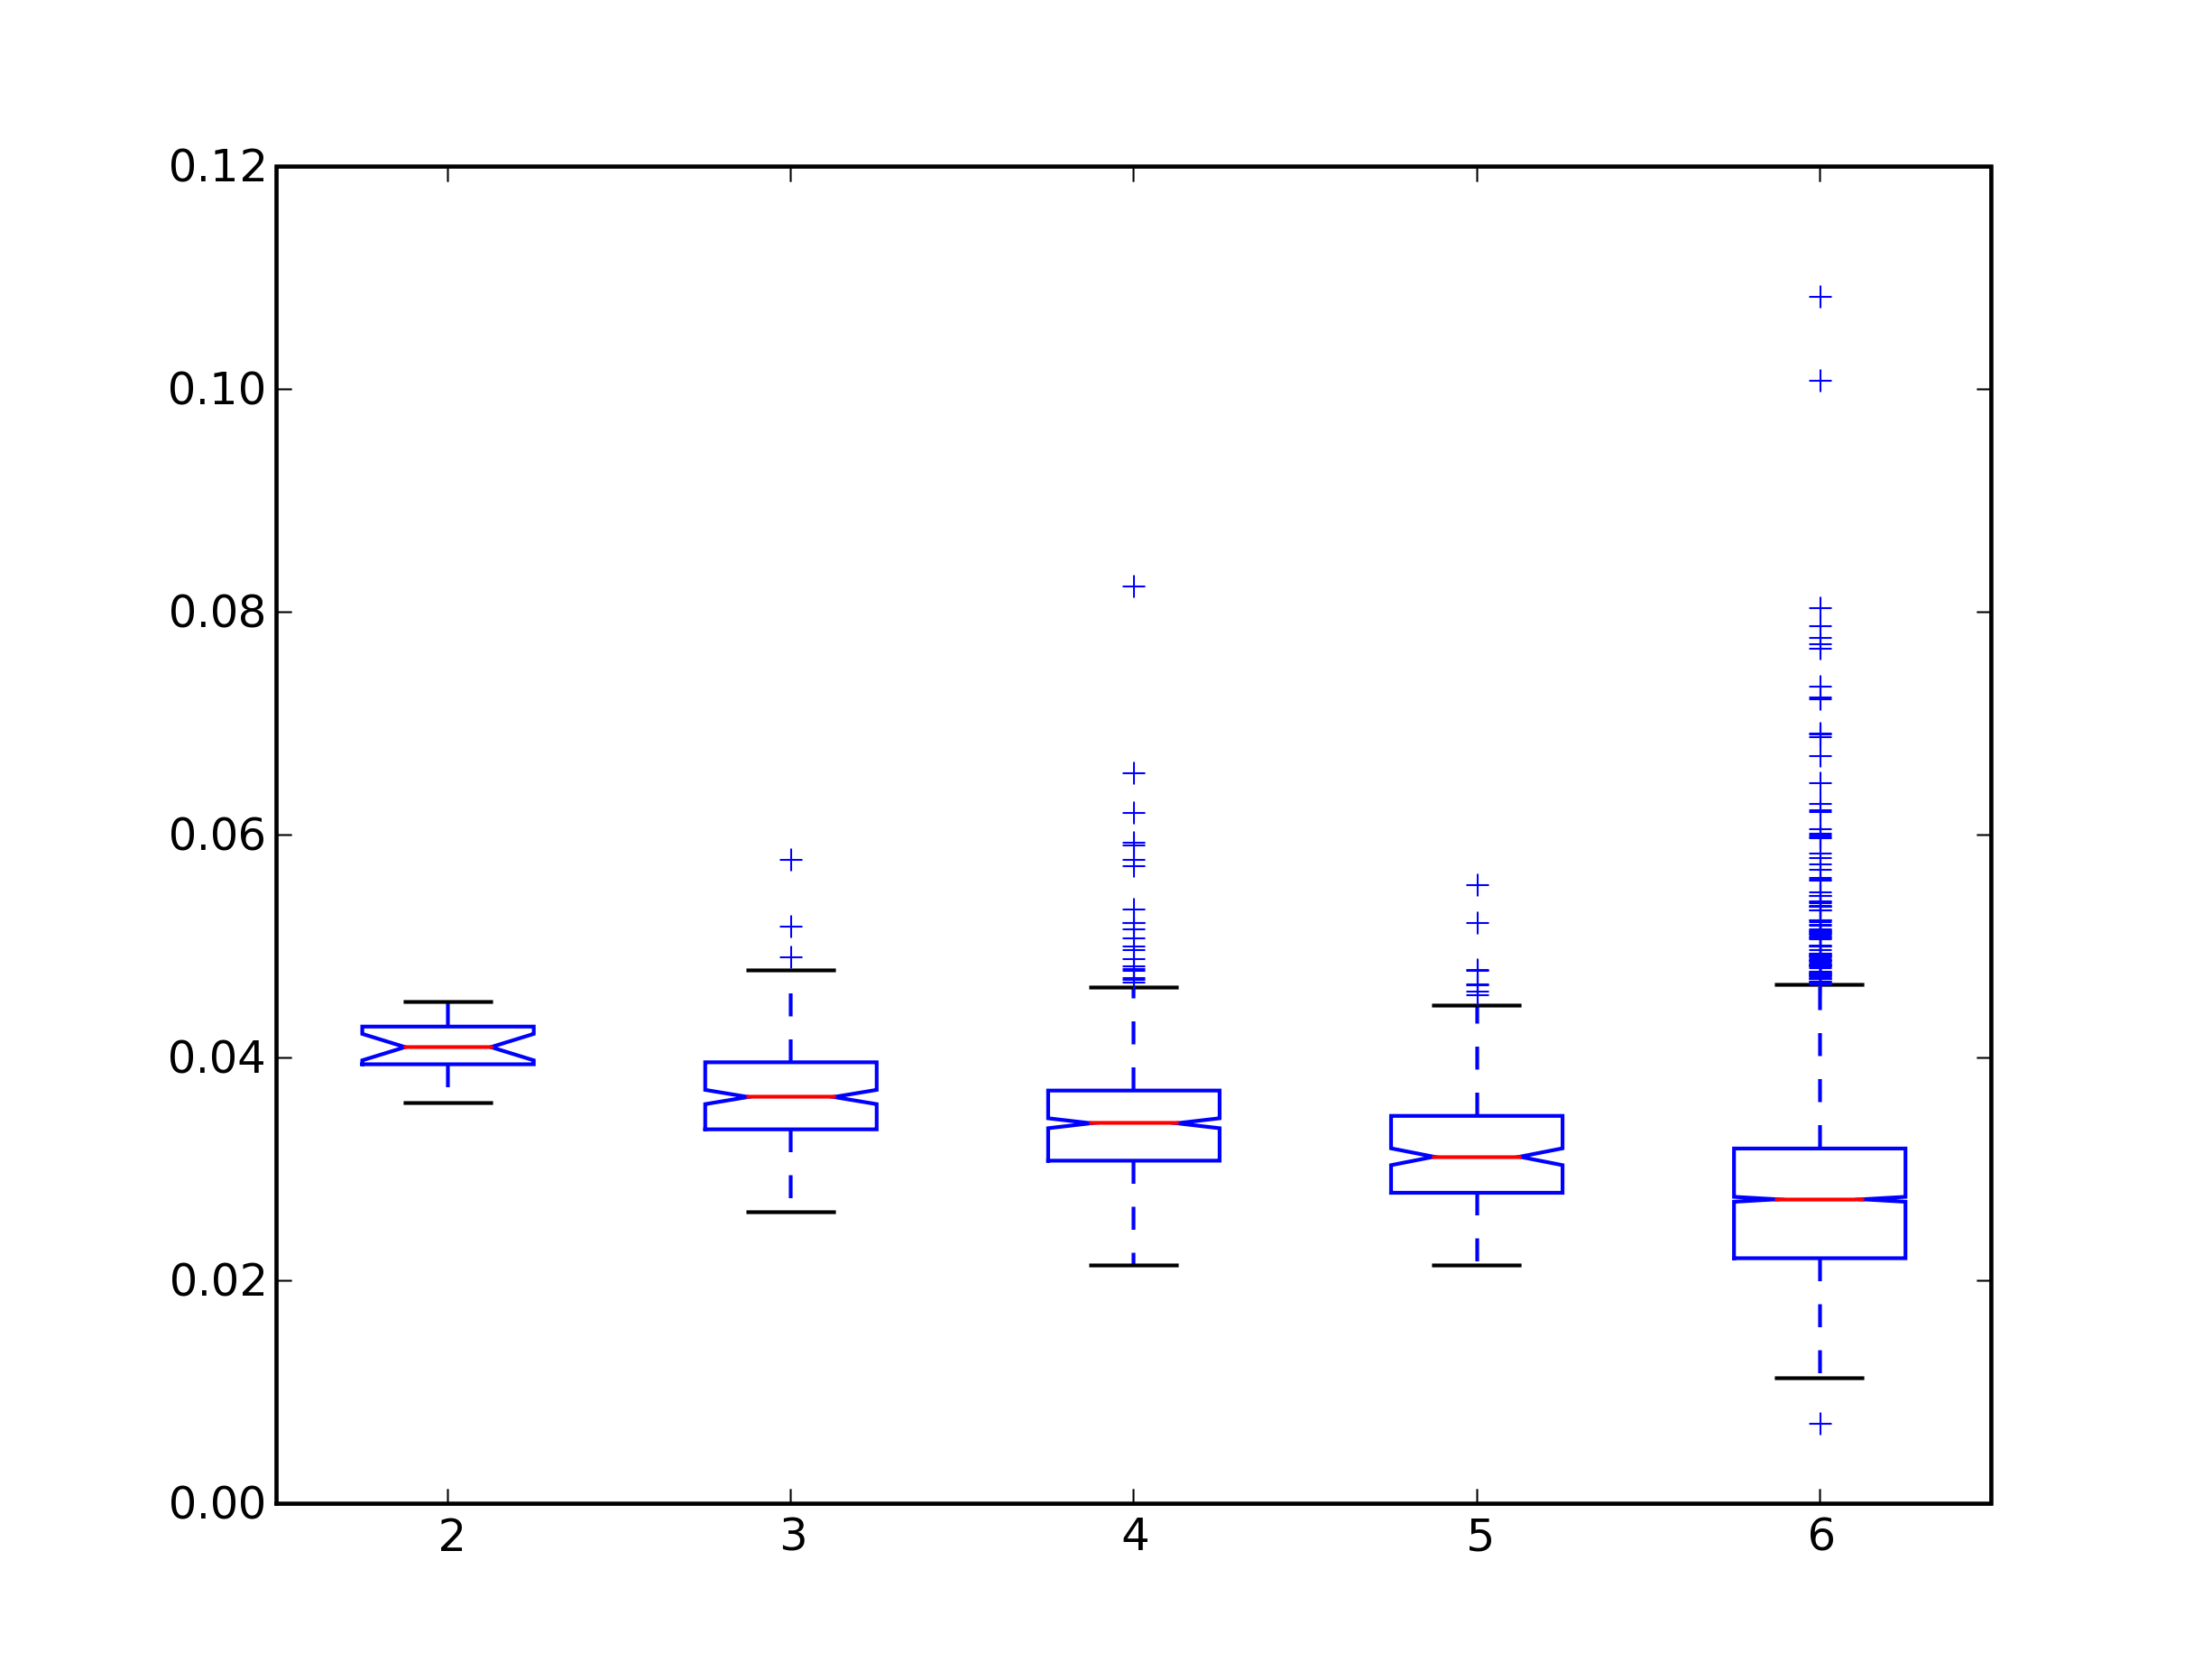
\includegraphics[width=.45\linewidth]{hex_iv_box.png}
}
\subfigure[Spherical Topology]{
  \label{boxplot:graph}
  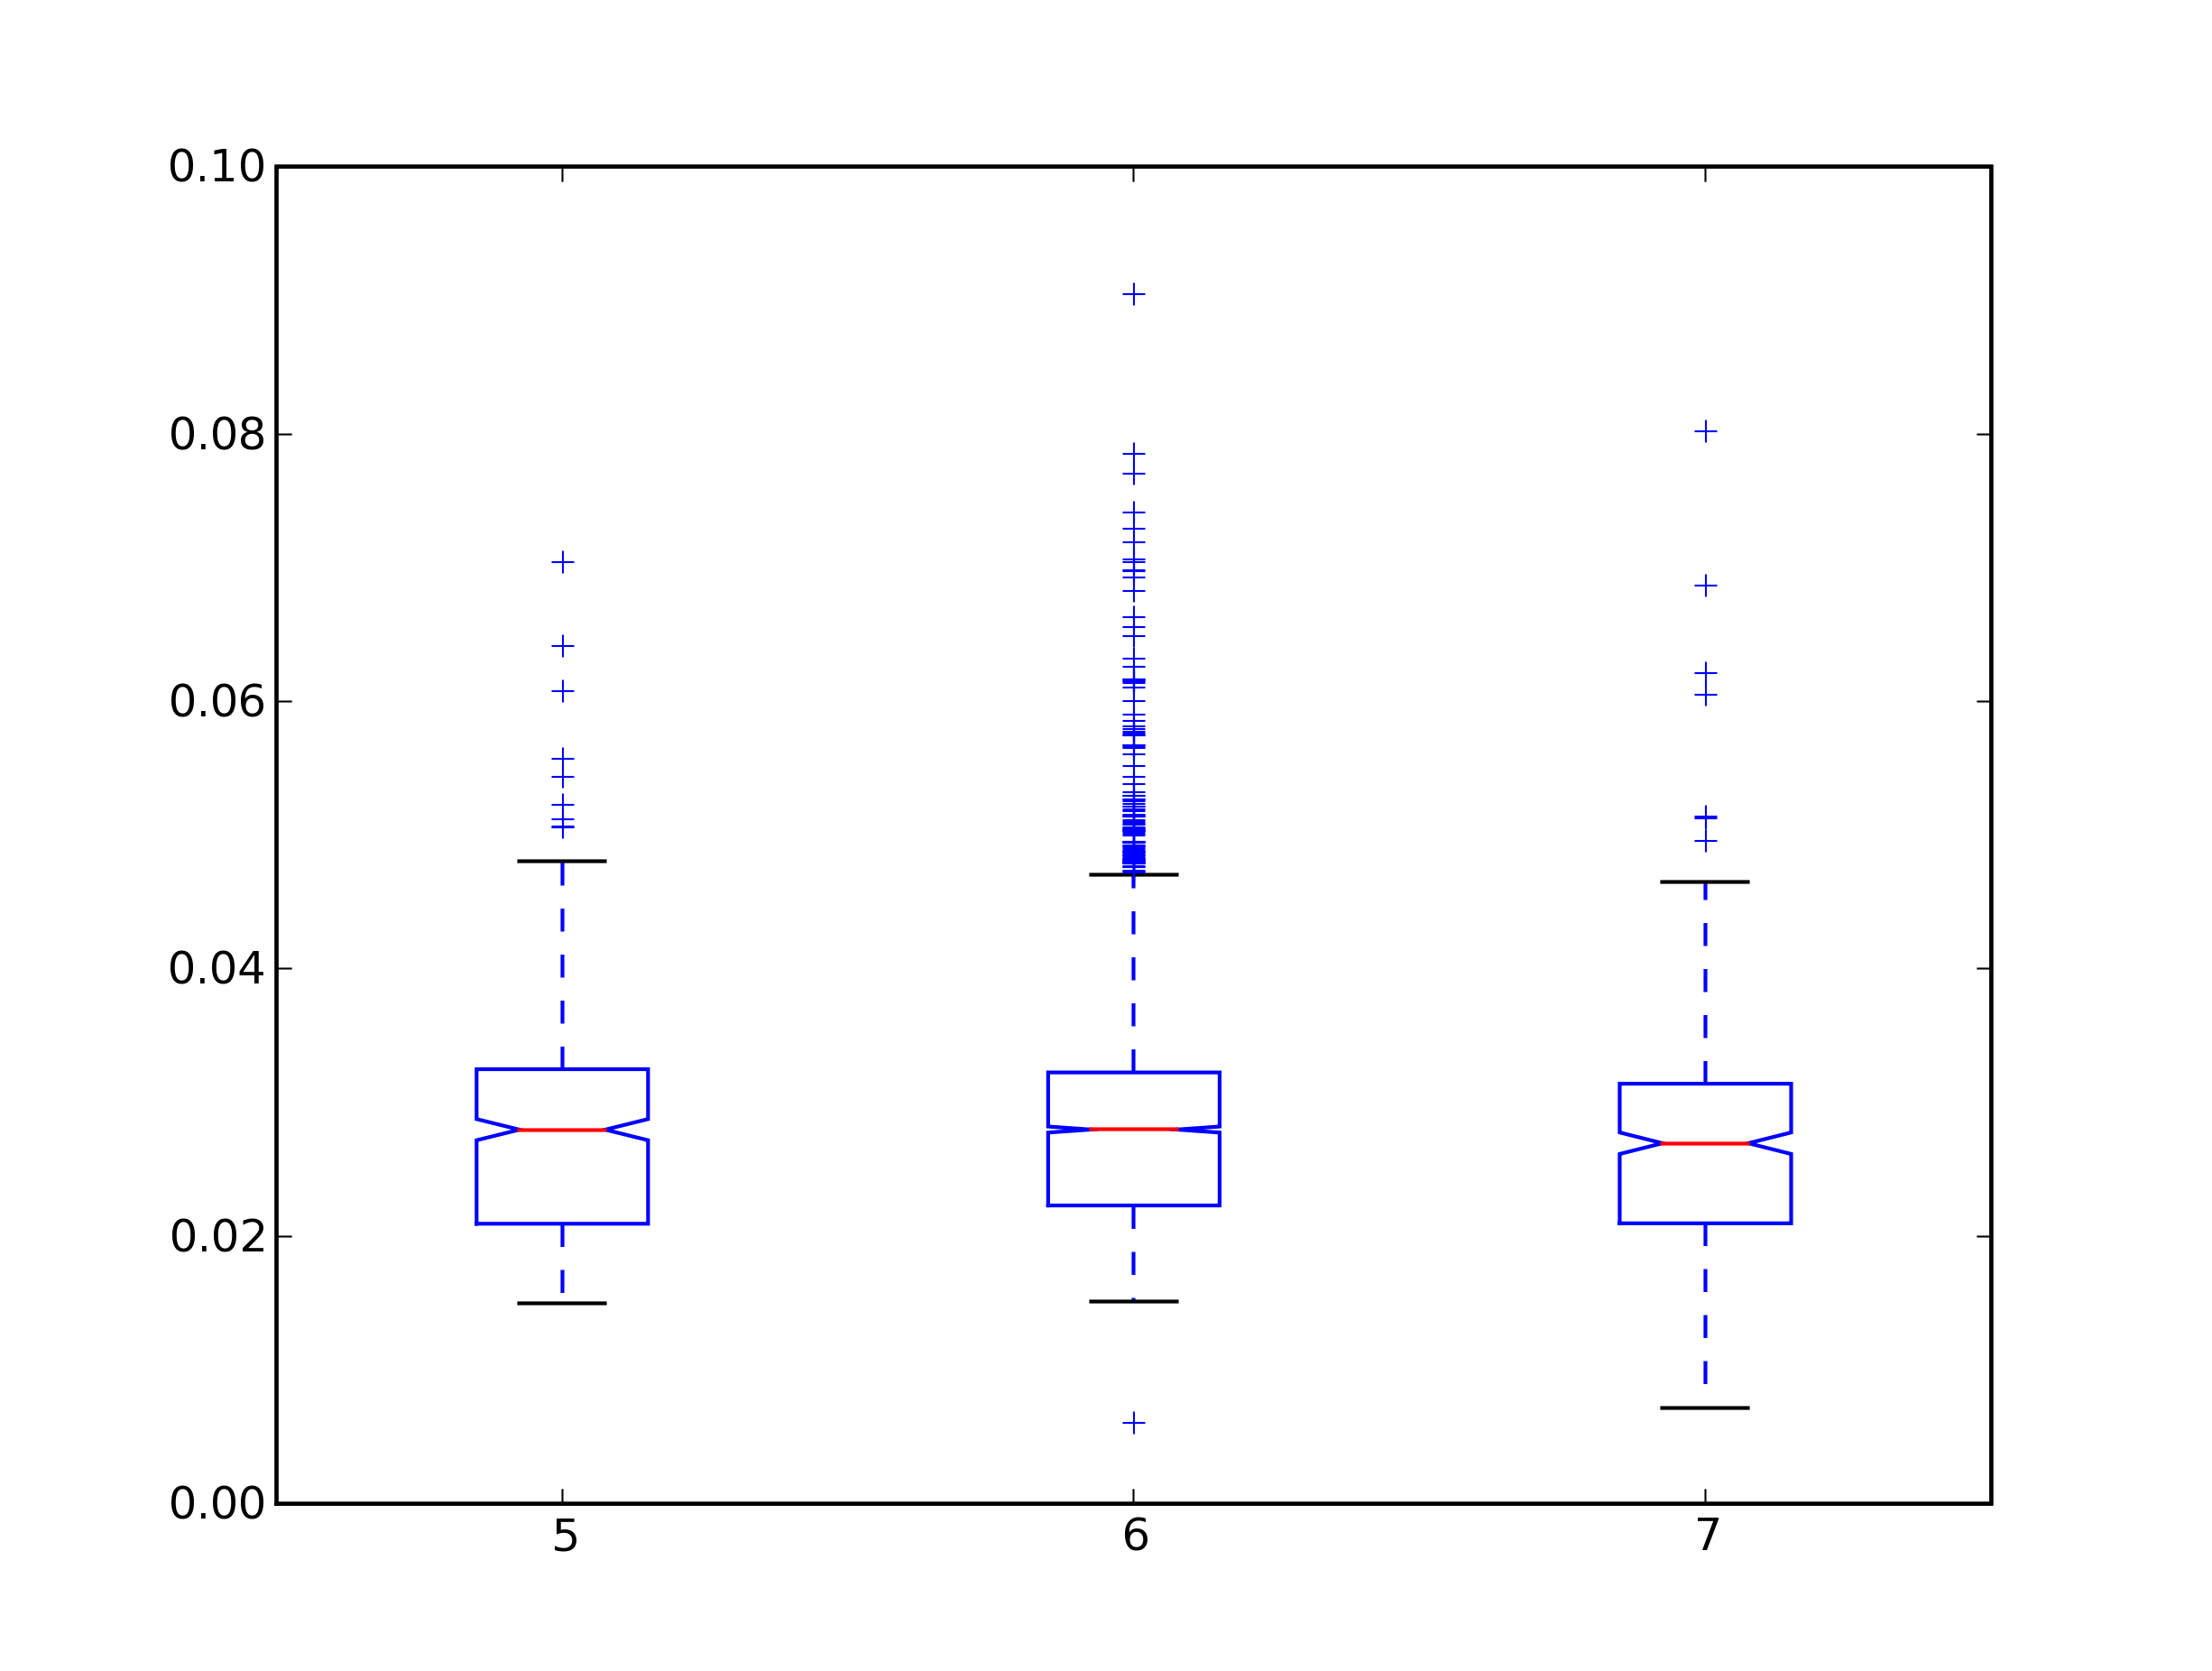
\includegraphics[width=.45\linewidth]{graph_iv_box.png}
}
\subfigure[Geodesic Sphere Topology]{
  \label{boxplot:geodesic}
  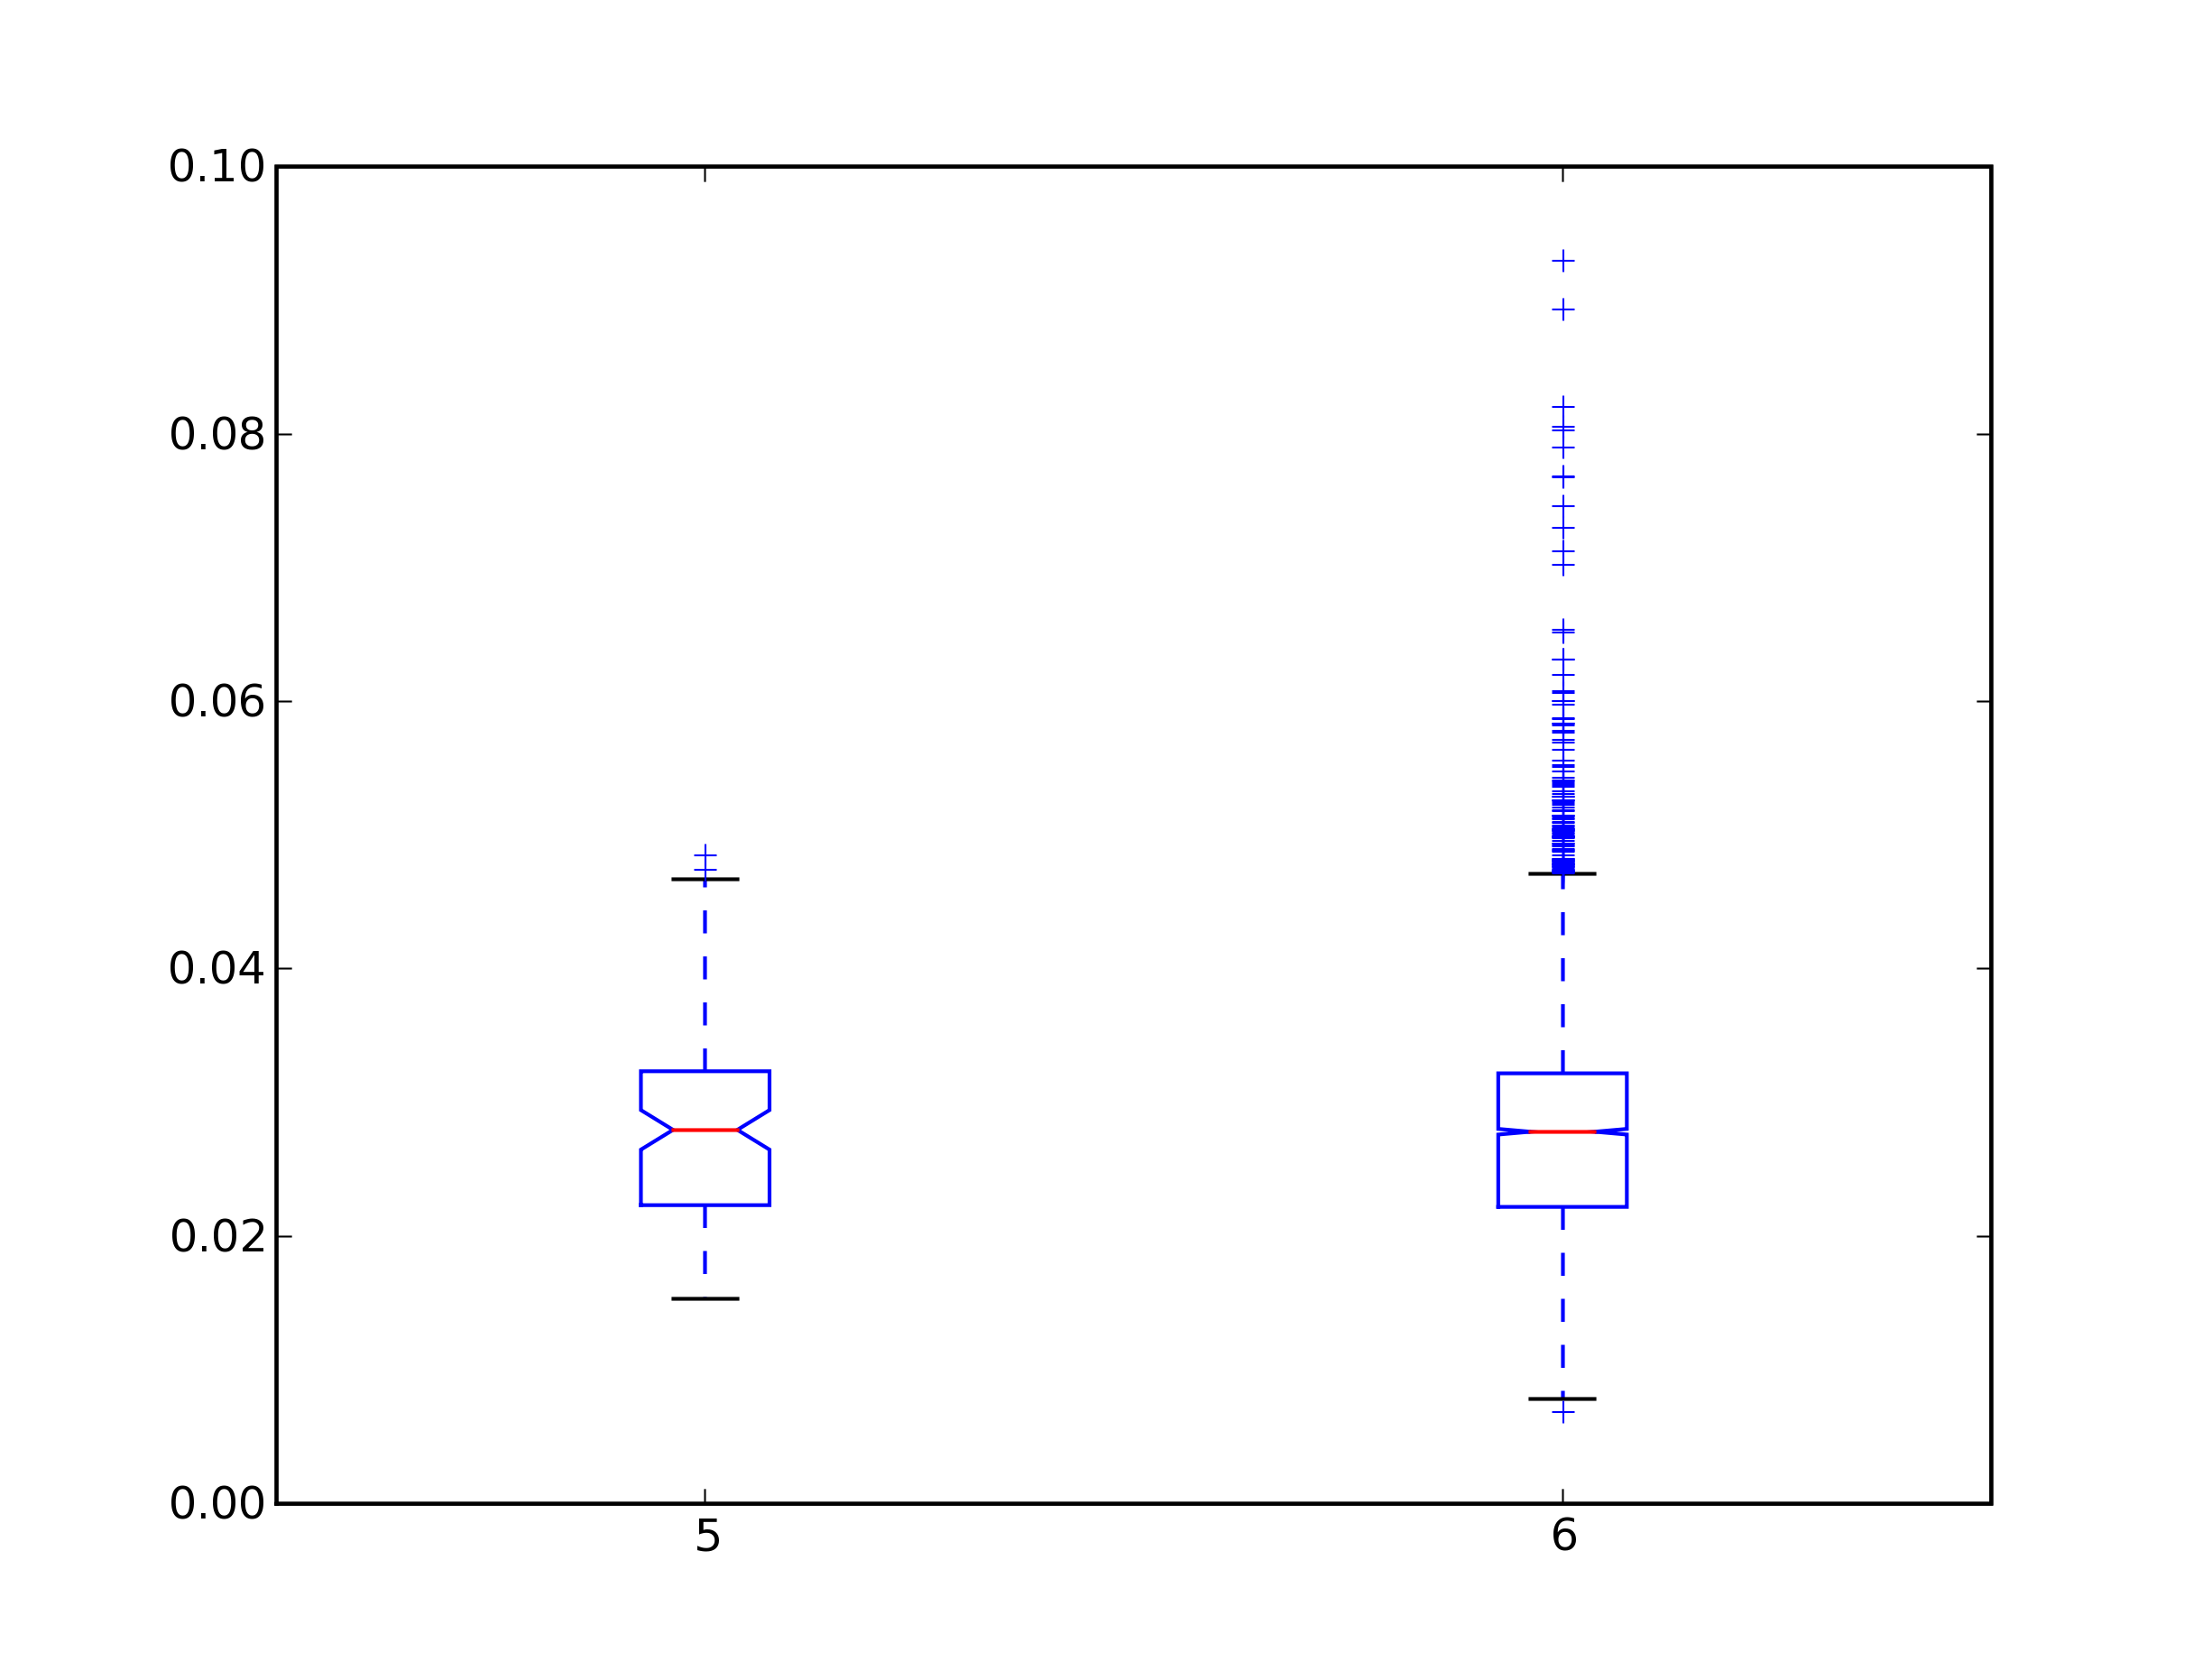
\includegraphics[width=.45\linewidth]{geodesic_iv_box.png}
}
\caption{This shows 4 box plots, each representing one group of neurons in a set
of SOMs trained with the same parameters.}
\label{boxplot}
\end{figure}

Table \ref{meanvar1} shows the mean internal variance for each group for each
topology. Again we see that the internal variances seem to respond as expected
in the ``flat'' topologies, but not in the spherical topologies.  This is not
necessarily bad, as it may suggest that the spherical topologies are
effectively overcoming the edge problem.  The difference between these means
and their significance is presented in tables \ref{rlt}.  For the rook
topology table \ref{rlt:rook} shows that its three groups are significantly
different from each other. Results are similar for the hexagonal topology. For
the Spherical and Geodesic Topologies however there is no significant
differance between the groups.
%I suspect a better measure would be to use the minimum number of steps for a
%given nueron to reach every other neuron on the network.  This would vary
%significantly on the rook and hexagon topolgoies, but not very much in the
%spherical topologies.

\begin{table}[hbt]
\caption{Mean IV and Var(IV) grouped by a neurons degree for each topology}
\label{meanvar1}
\begin{tabular}{|c||c|c||c|c||c|c||c|c|}
\hline
\textbf{Degree Size} & \multicolumn{2}{c||}{\textbf{Geodesic}} &
\multicolumn{2}{c||}{\textbf{Spherical}} & \multicolumn{2}{c||}{\textbf{Hex}} &
\multicolumn{2}{c||}{\textbf{Rook}} \\
\hline
& N & Mean (Var) & N & Mean (Var) & N & Mean (Var) & N & Mean (Var) \\
\hline
2&&&&& 20& 0.0611 (0.0013)& 40& 0.1095 (0.0040)\\ 
3&&&&& 230& 0.0790 (0.0024)& 939& 0.0821 (0.0027)\\ 
4&&&&& 520& 0.0852 (0.0029)& 5446& 0.0484 (0.0013)\\ 
5& 120& 0.0536 (0.0015)& 589& 0.0563 (0.0016)& 210& 0.0666 (0.0027)&&\\ 
6& 6287& 0.0548 (0.0015)& 5349& 0.0543 (0.0015)& 5448& 0.0495 (0.0014)&&\\ 
7&&& 469& 0.0567 (0.0015)&&&&\\ 
\hline
\end{tabular} \end{table}



%\subsection{Restate the Questions}
%\textbf{Objective}, Compare the internal variance of observations captured by a given
%neuron to that neuron's first-order neighborhood size.
%\textbf{Question}, Does the internal variance of a neuron decrease as its first-order
%neighborhood size, or degree, increases?


\begin{table}[hbt]
\centering
\caption{These tables show the difference in mean IV between each group of
neurons grouped by their degree, delta (significance),
t=9999, *** = 99\%, ** = 95\%, * = 90\%}
\label{rlt}


  \subtable[Rook Topology]{
    \label{rlt:rook}
    \begin{tabular}{|c||c|c|c|}
    \hline
    Degree&2&3&4\\\hline
    \hline
    2 & (0.004008) & \textbf{0.001000} & \textbf{0.001000}\\\hline
    3 & 0.027352 & (0.002723) & \textbf{0.001000}\\\hline
    4 & 0.061040 & 0.033688 & (0.001287)\\\hline
    \end{tabular}
  }

  \subtable[Hexagonal Topology]{
    \label{rlt:hex}
    \begin{tabular}{|c||c|c|c|c|c|}
    \hline
    Degree&2&3&4&5&6\\ \hline
    \hline
     2 & (0.001304) & 0.115000 & \textbf{0.046000} & 0.646000 & 0.166000\\\hline
     3 & 0.017918 & (0.002389) & 0.148000 & \textbf{0.013000} & \textbf{0.001000}\\\hline
     4 & 0.024169 & 0.006251 & (0.002866) & \textbf{0.001000} & \textbf{0.001000}\\\hline
     5 & 0.005528 & 0.012389 & 0.018640 & (0.002678) & \textbf{0.001000}\\\hline
     6 & 0.011560 & 0.029478 & 0.035729 & 0.017089 & (0.001402)\\\hline
    \end{tabular}
  }

  \subtable[Spherical Topology]{
    \label{rlt:graph}
    \begin{tabular}{|c||c|c|c|}
    \hline	
    Degree&5&6&7\\ \hline
    \hline
     5 & (0.001583) & 0.225000 & 0.857000\\\hline
     6 & 0.001941 & (0.001474) & 0.201000\\\hline
     7 & 0.000462 & 0.002402 & (0.001472)\\\hline
    \end{tabular}
  }

  \subtable[Geodesic Topology]{
    \label{rlt:geodesic}
    \begin{tabular}{|c||c|c|}
    \hline
    Degree&5&6\\ \hline
    \hline
     5 & (0.001466) & 0.724000\\\hline
     6 & 0.001227 & (0.001494)\\\hline
    \end{tabular}
  }
\end{table}

\subsection{Internal variance vs. centrality}
Above we saw that changes in a neuron's degree was related to changes in
internal variance in topologies with edges, but not in the two sphere based
topologies. The next step is to see if internal variance changes between
topologies.  To do this we will first order out topologies by a summary
measure of the network centrality.  A node's centrality can be thought of as a
measure of it's importance to the rest of the network. Above we used the most
common measure of centrality, which is a node's degree.  For this diagnostic
we'll take the variance of those degrees as a summary measure.  This should
tell us how regular the overall network is.  These variances and the sorting
of our topologies is shown in table \ref{vardeg}.

\begin{table}[hbt]
\centering
\caption{This table shows how our topologies will be sorted based on the
variance in degrees of the topology's nodes}
\label{vardeg}
\begin{tabular}{|c|c|c|c|}
\hline
Topology & Var of Degree & MeanIV (VarIV)\\
\hline
Geodesic & 0.0183 & 0.0874 (0.0009)\\
Rook & 0.1457 & 0.0890 (0.0010)\\
Spherical & 0.1648 & 0.0879 (0.0010)\\
Hexagonal & 0.6283 & 0.0885 (0.0010)\\
\hline
\end{tabular}
\end{table}

Figure \ref{q2boxplot} shows the distribution on internal variance
measurements for each of our topologies.  It is interesting to note that
they all appear to be very similar. We test the difference in means for
each of these using the same method of random labeling that was applied in the
previous diagnostic. The results are displayed in table \ref{rlt:all}. Table
\ref{rlt:allV} shows the result of testing for a difference in variance
between each topology.  It was expected that the mean and variance of IV would
increase in more irregular topologies.  These result general do not support
that hypothesis. This may suggest that the mean and variance of IV are not
appropriate summary measures.

\begin{figure}[hbt]
\centering
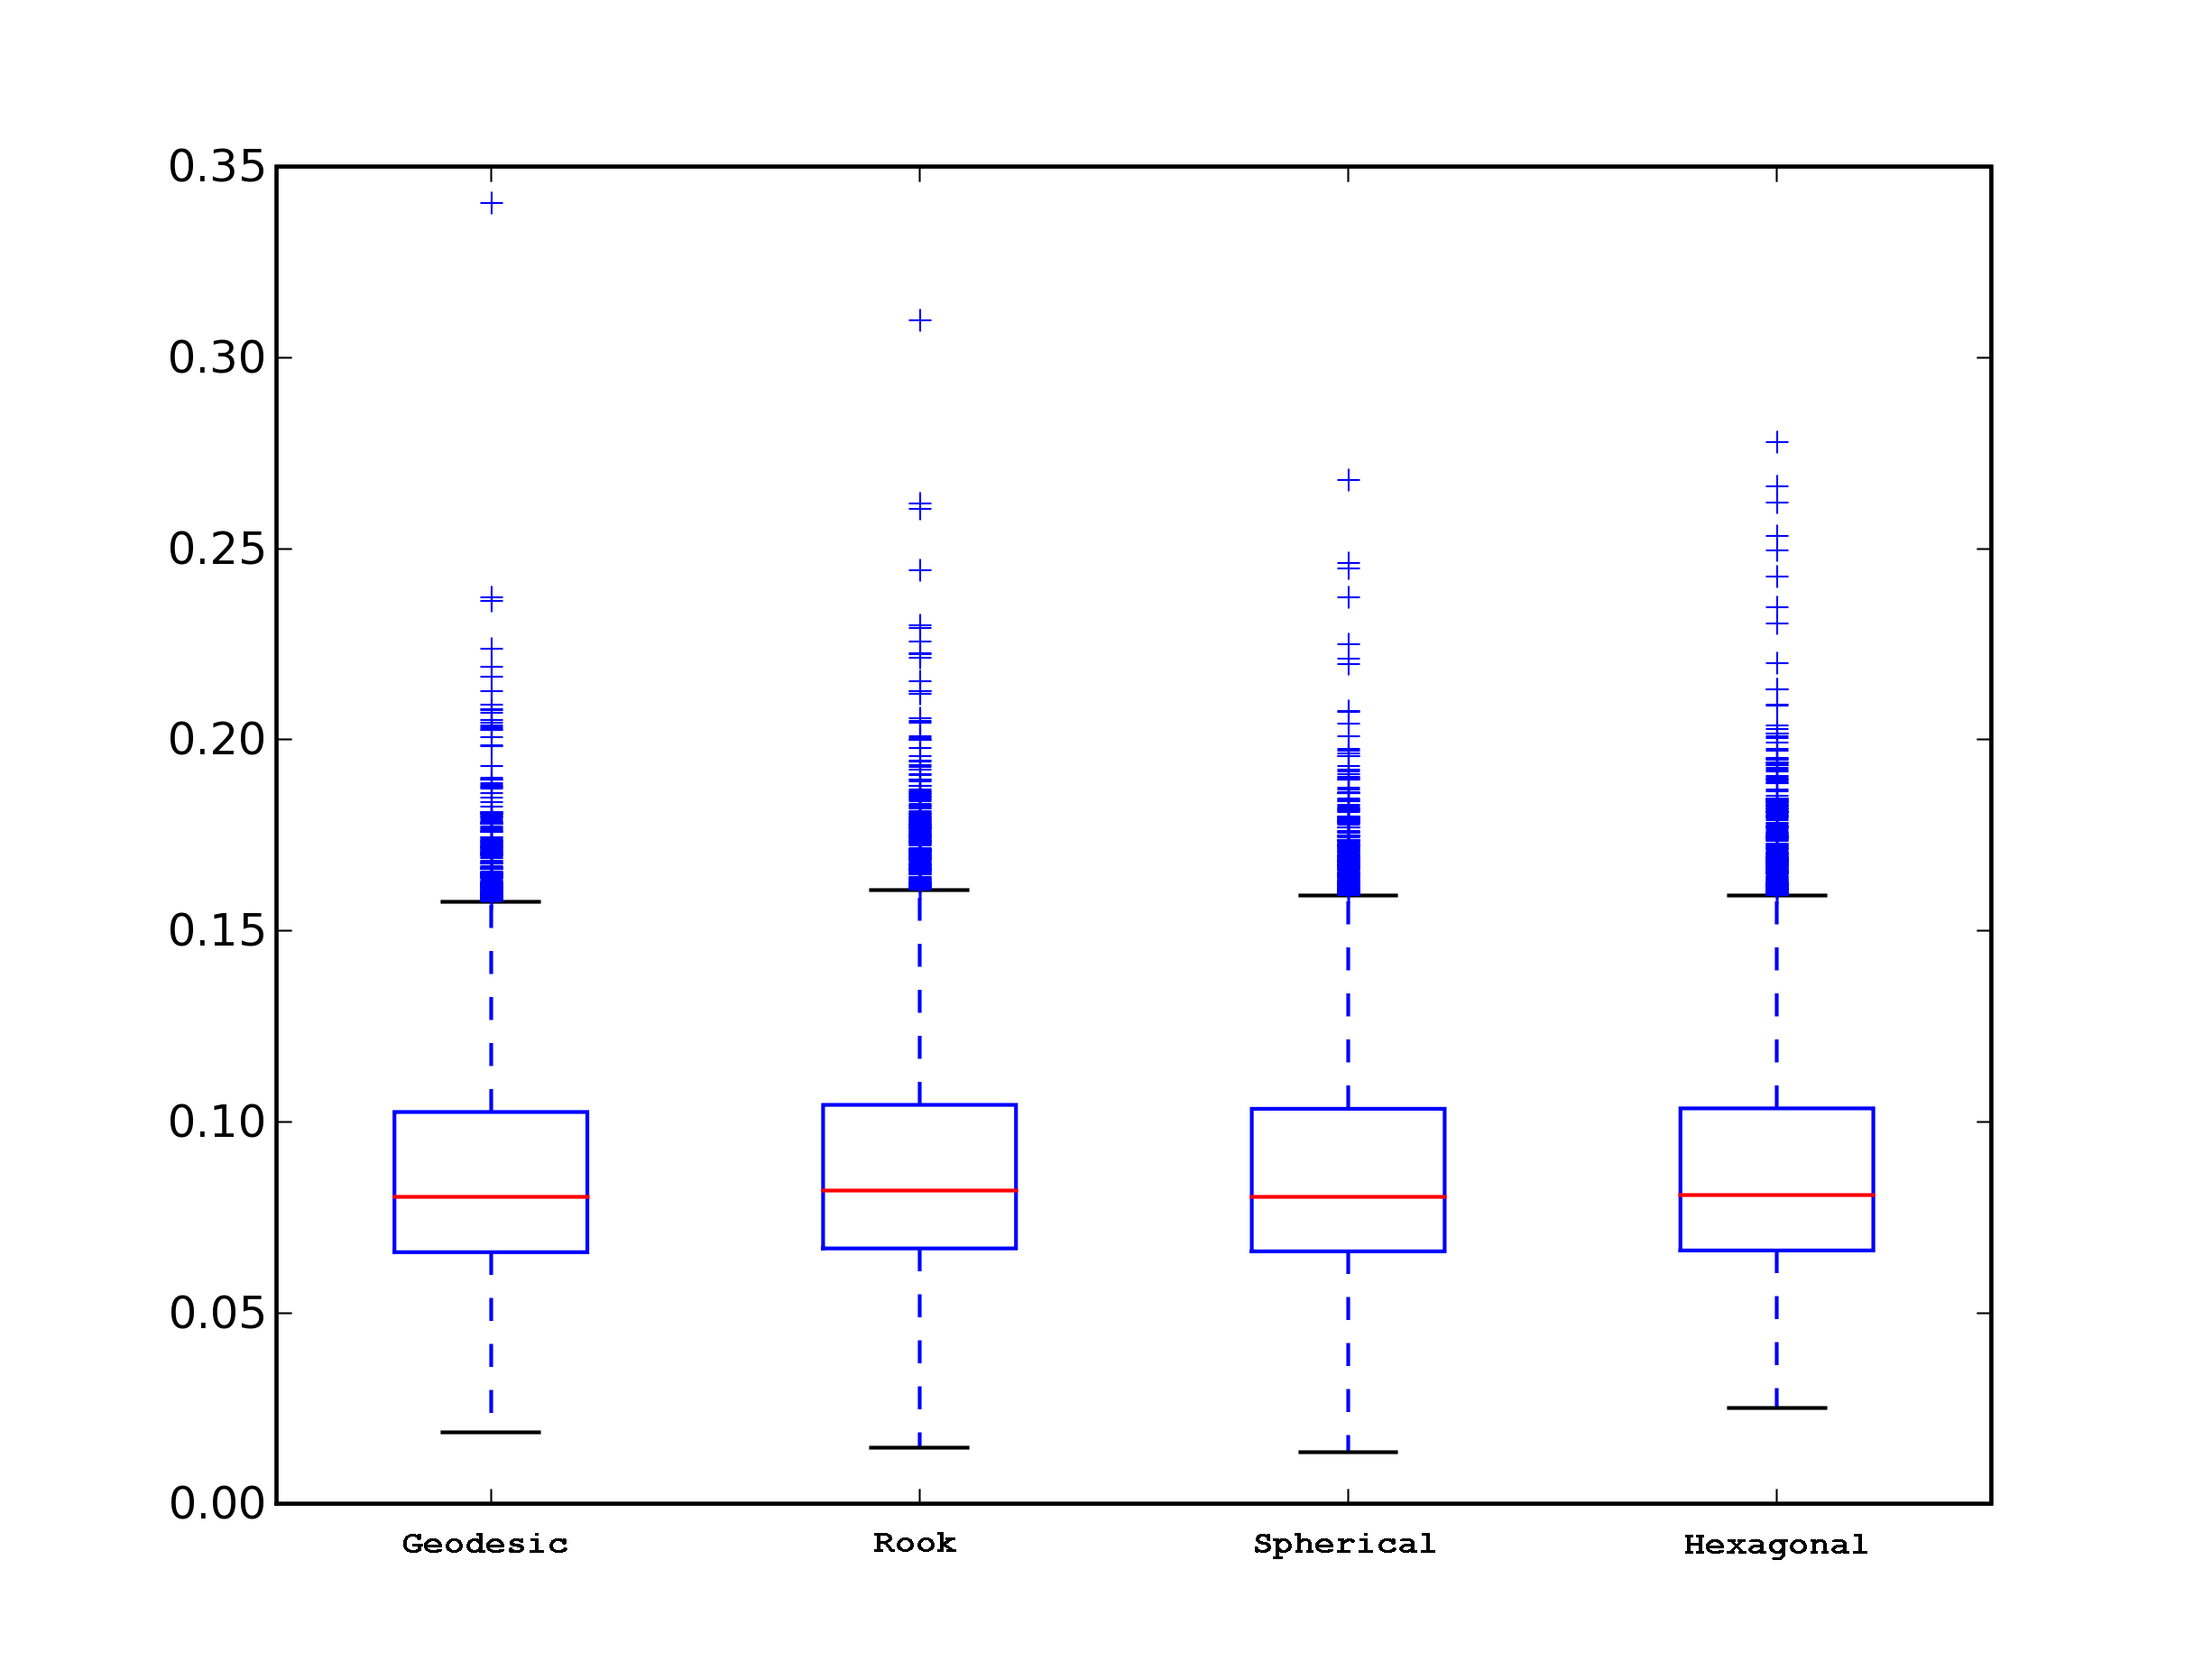
\includegraphics[width=\linewidth]{q2boxplot.png}
\caption{These box plots show the distribution of internal variance measurements
for each topology.}
\label{q2boxplot}
\end{figure}


\begin{table}[hbt]
  \centering
  \caption{These tables show the difference in means of the internal variance between each topology}
  \label{rlt:all}
  \begin{tabular}{|c||c|c|c|c|}
  \hline
  \textbf{Topology}&Geodesic &Rook	&Sphere			&Hexagonal		\\\hline
  \hline
  Geodesic	&& \textbf{0.0015} ***	& 0.0005		& \textbf{0.0010} *	\\\hline
  Rook		&& 			& \textbf{0.0011} *	& 0.0005		\\\hline
  Sphere	&& 			& 			& 0.0005 		\\\hline
  Hexagonal 	&& 			& 			&			\\\hline
  \end{tabular}
  \end{table}




\begin{table}[hbt]
  \centering
  \caption{These tables show the difference in variances of the internal variance between each topology}
  \label{rlt:allV}
  \begin{tabular}{|c||c|c|c|c|}
  \hline
  \textbf{Topology}&Geodesic &Rook	&Sphere			&Hexagonal		\\\hline
  \hline
  Geodesic	&& \textbf{0.0009} *	& 0.0003		& \textbf{0.0011} **	\\\hline
  Rook		&& 			& 0.0005		& 0.0002		\\\hline
  Sphere	&& 			& 			& 0.0007 		\\\hline
  Hexagonal 	&& 			& 			&			\\\hline
  \end{tabular}
  \end{table}



\subsection{Visualization of Internal Variance}
In this section we will look at what information can be gained from
visualizing the SOM and its internal variance. The visualizations are created
with off the shelf GIS packages, namely ESRI's ArcGIS.  There are a number of
challenges which must be overcome before one can visualize the SOM.  To
visualize the rook and hexagonal topologies we simply need to create polygons
centered over each neuron.  The spherical and geodesic topologies are slightly
more complicated.  To create the polygons for these topologies we must first
compute the voronoi diagram on the surface of the sphere.  This is done using
``STRIPACK'', a software program created by \cite{Ranka97}.  The next problem
is that ArcGIS and other common GIS packages assume Cartesian distances.  They
can not handle polygons that cross the $180^{th}$ meridian.  To accommodate this we
must split each polygon at the $180^{th}$ meridian and draw it as two parts.  This
is done by checking each edge of each polygon to see if it crosses this
meridian, if it does we calculate its intersection with the meridian and split
the edge into two segments.

        Figure \ref{ten} shows cool stuff.





%\begin{figure}[hbt]
%	\centering
%	\includegraphics[width=\linewidth]{geo_poly.png}
%	\caption{This is a visualiation of the internal variance on the
%Geodesic SOM.}
%	\label{geopoly}
%\end{figure}

\begin{figure}[hbt]
\centering
\subfigure[Rook Topology]{
  \label{ten:rook}
  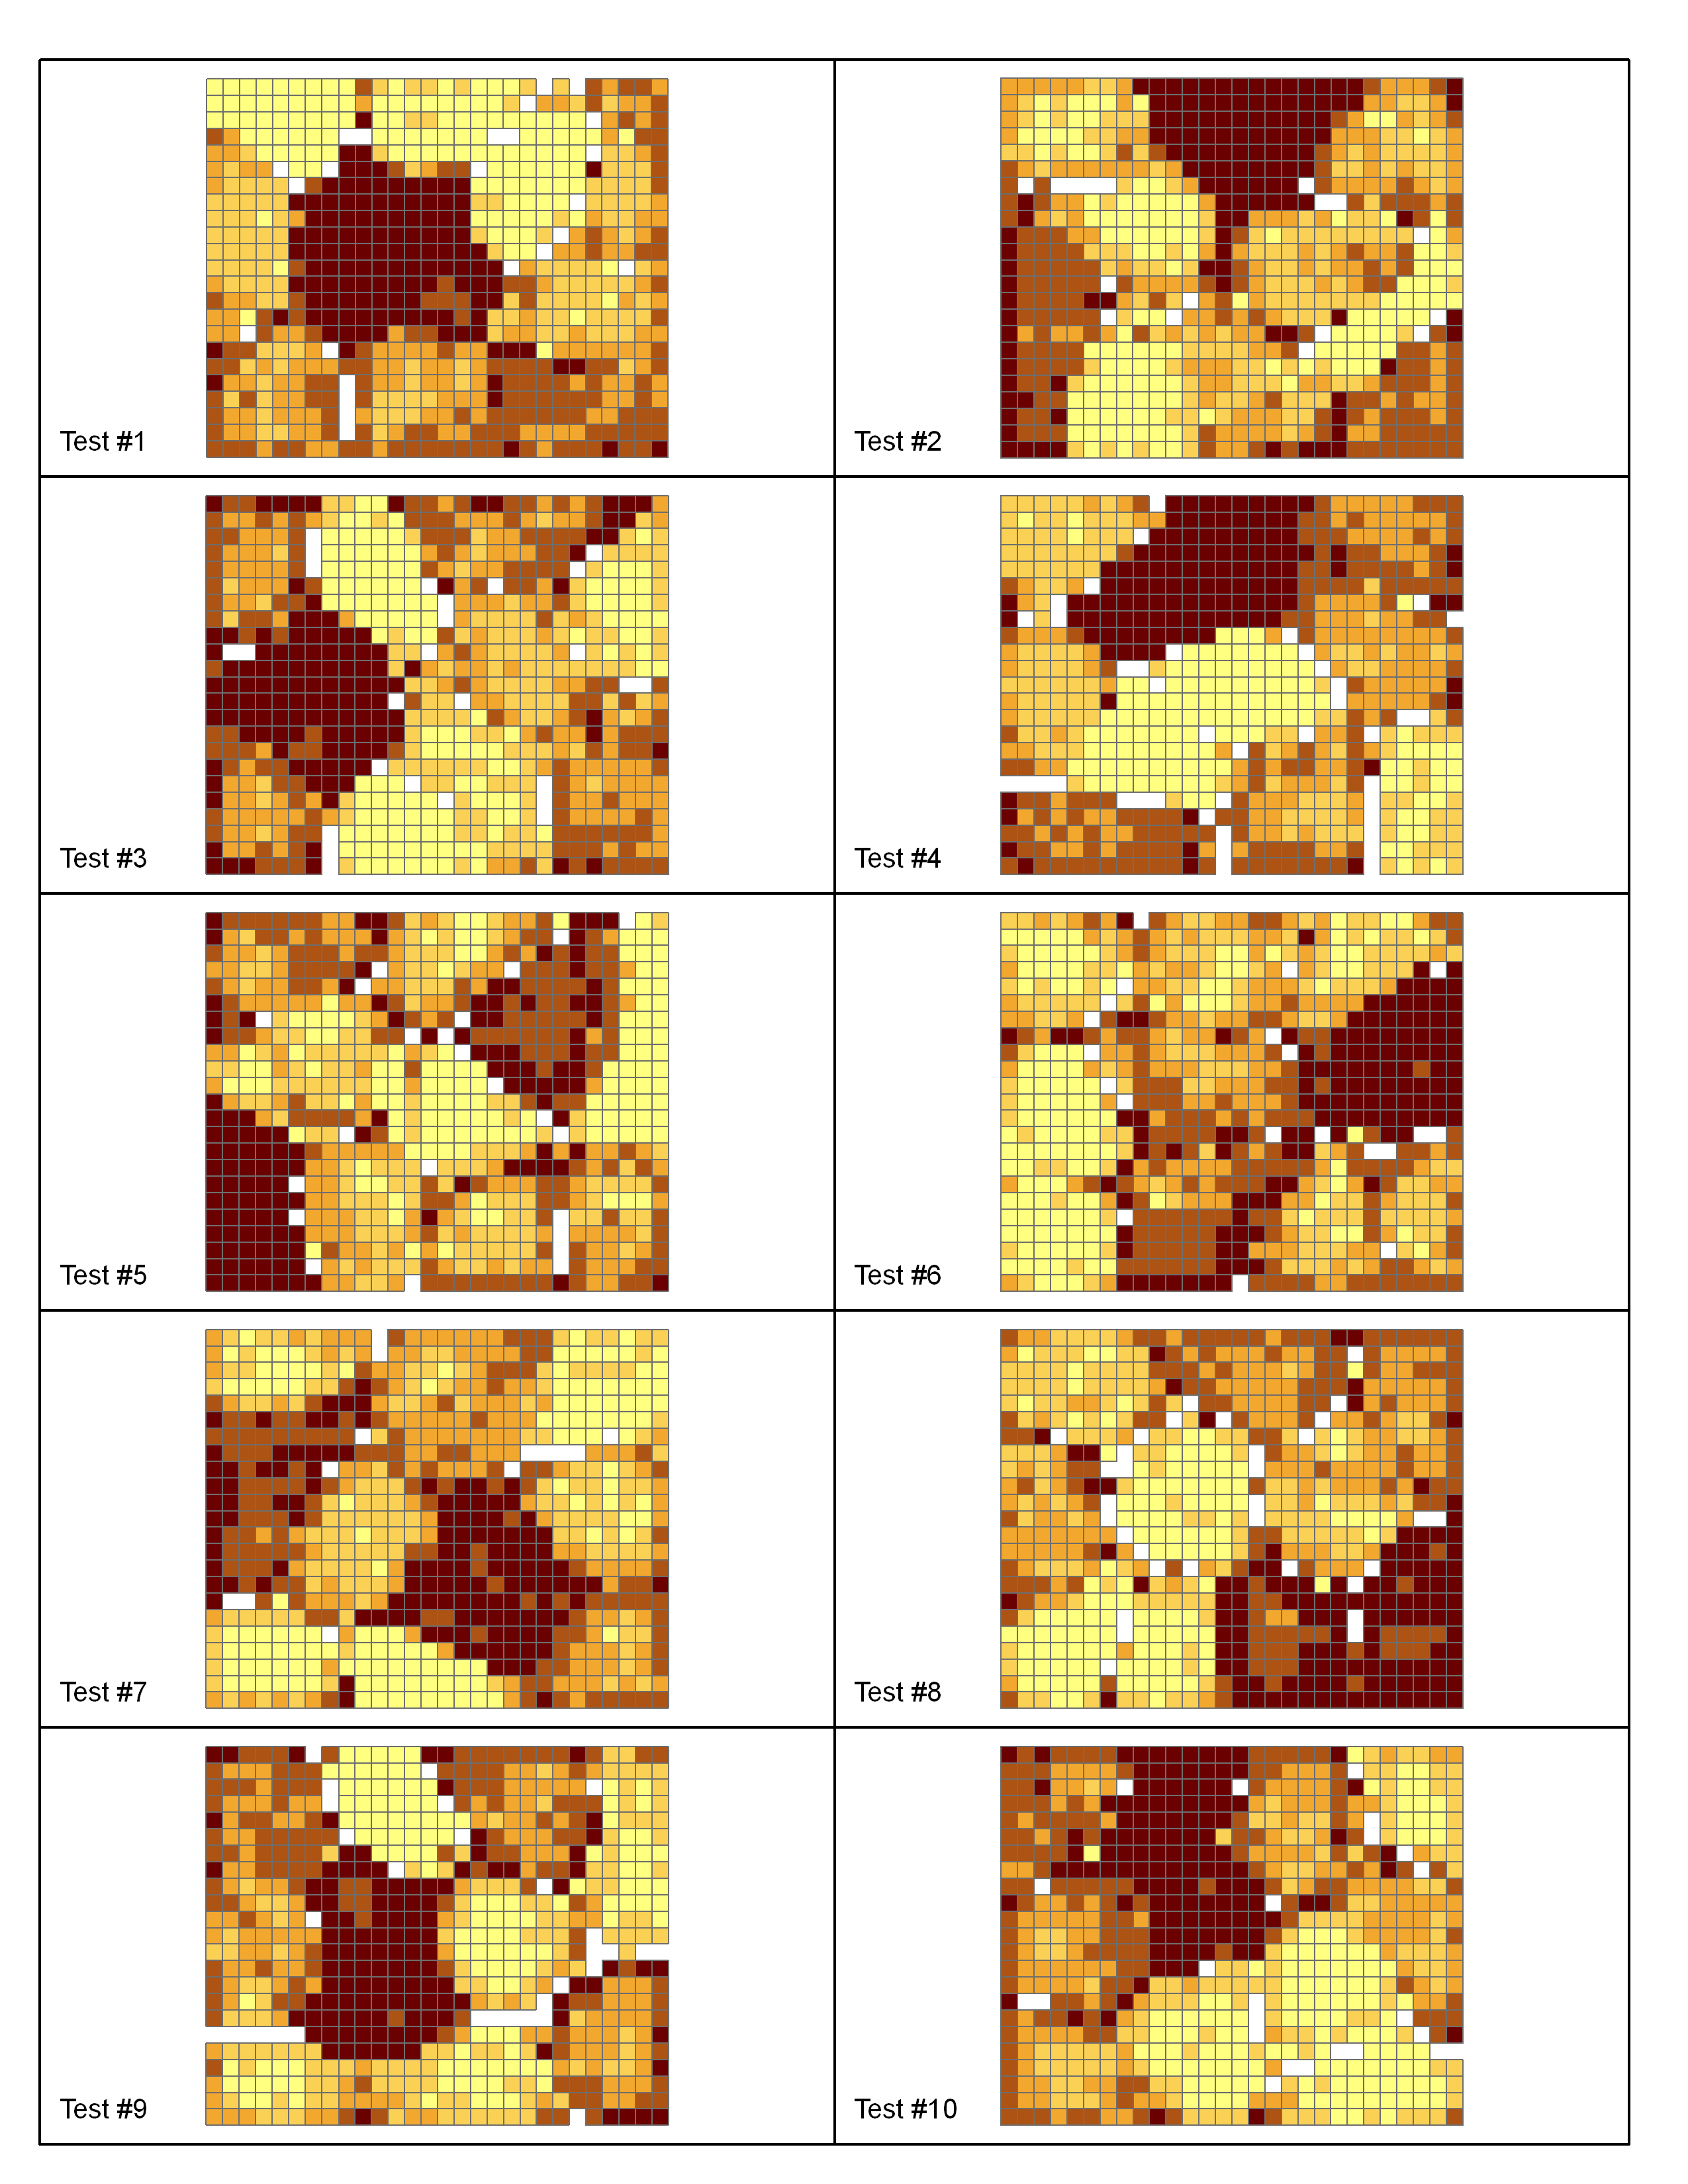
\includegraphics[width=.40\linewidth]{rook_10.png}
}
\subfigure[Hexagonal Topology]{
  \label{ten:hex}
  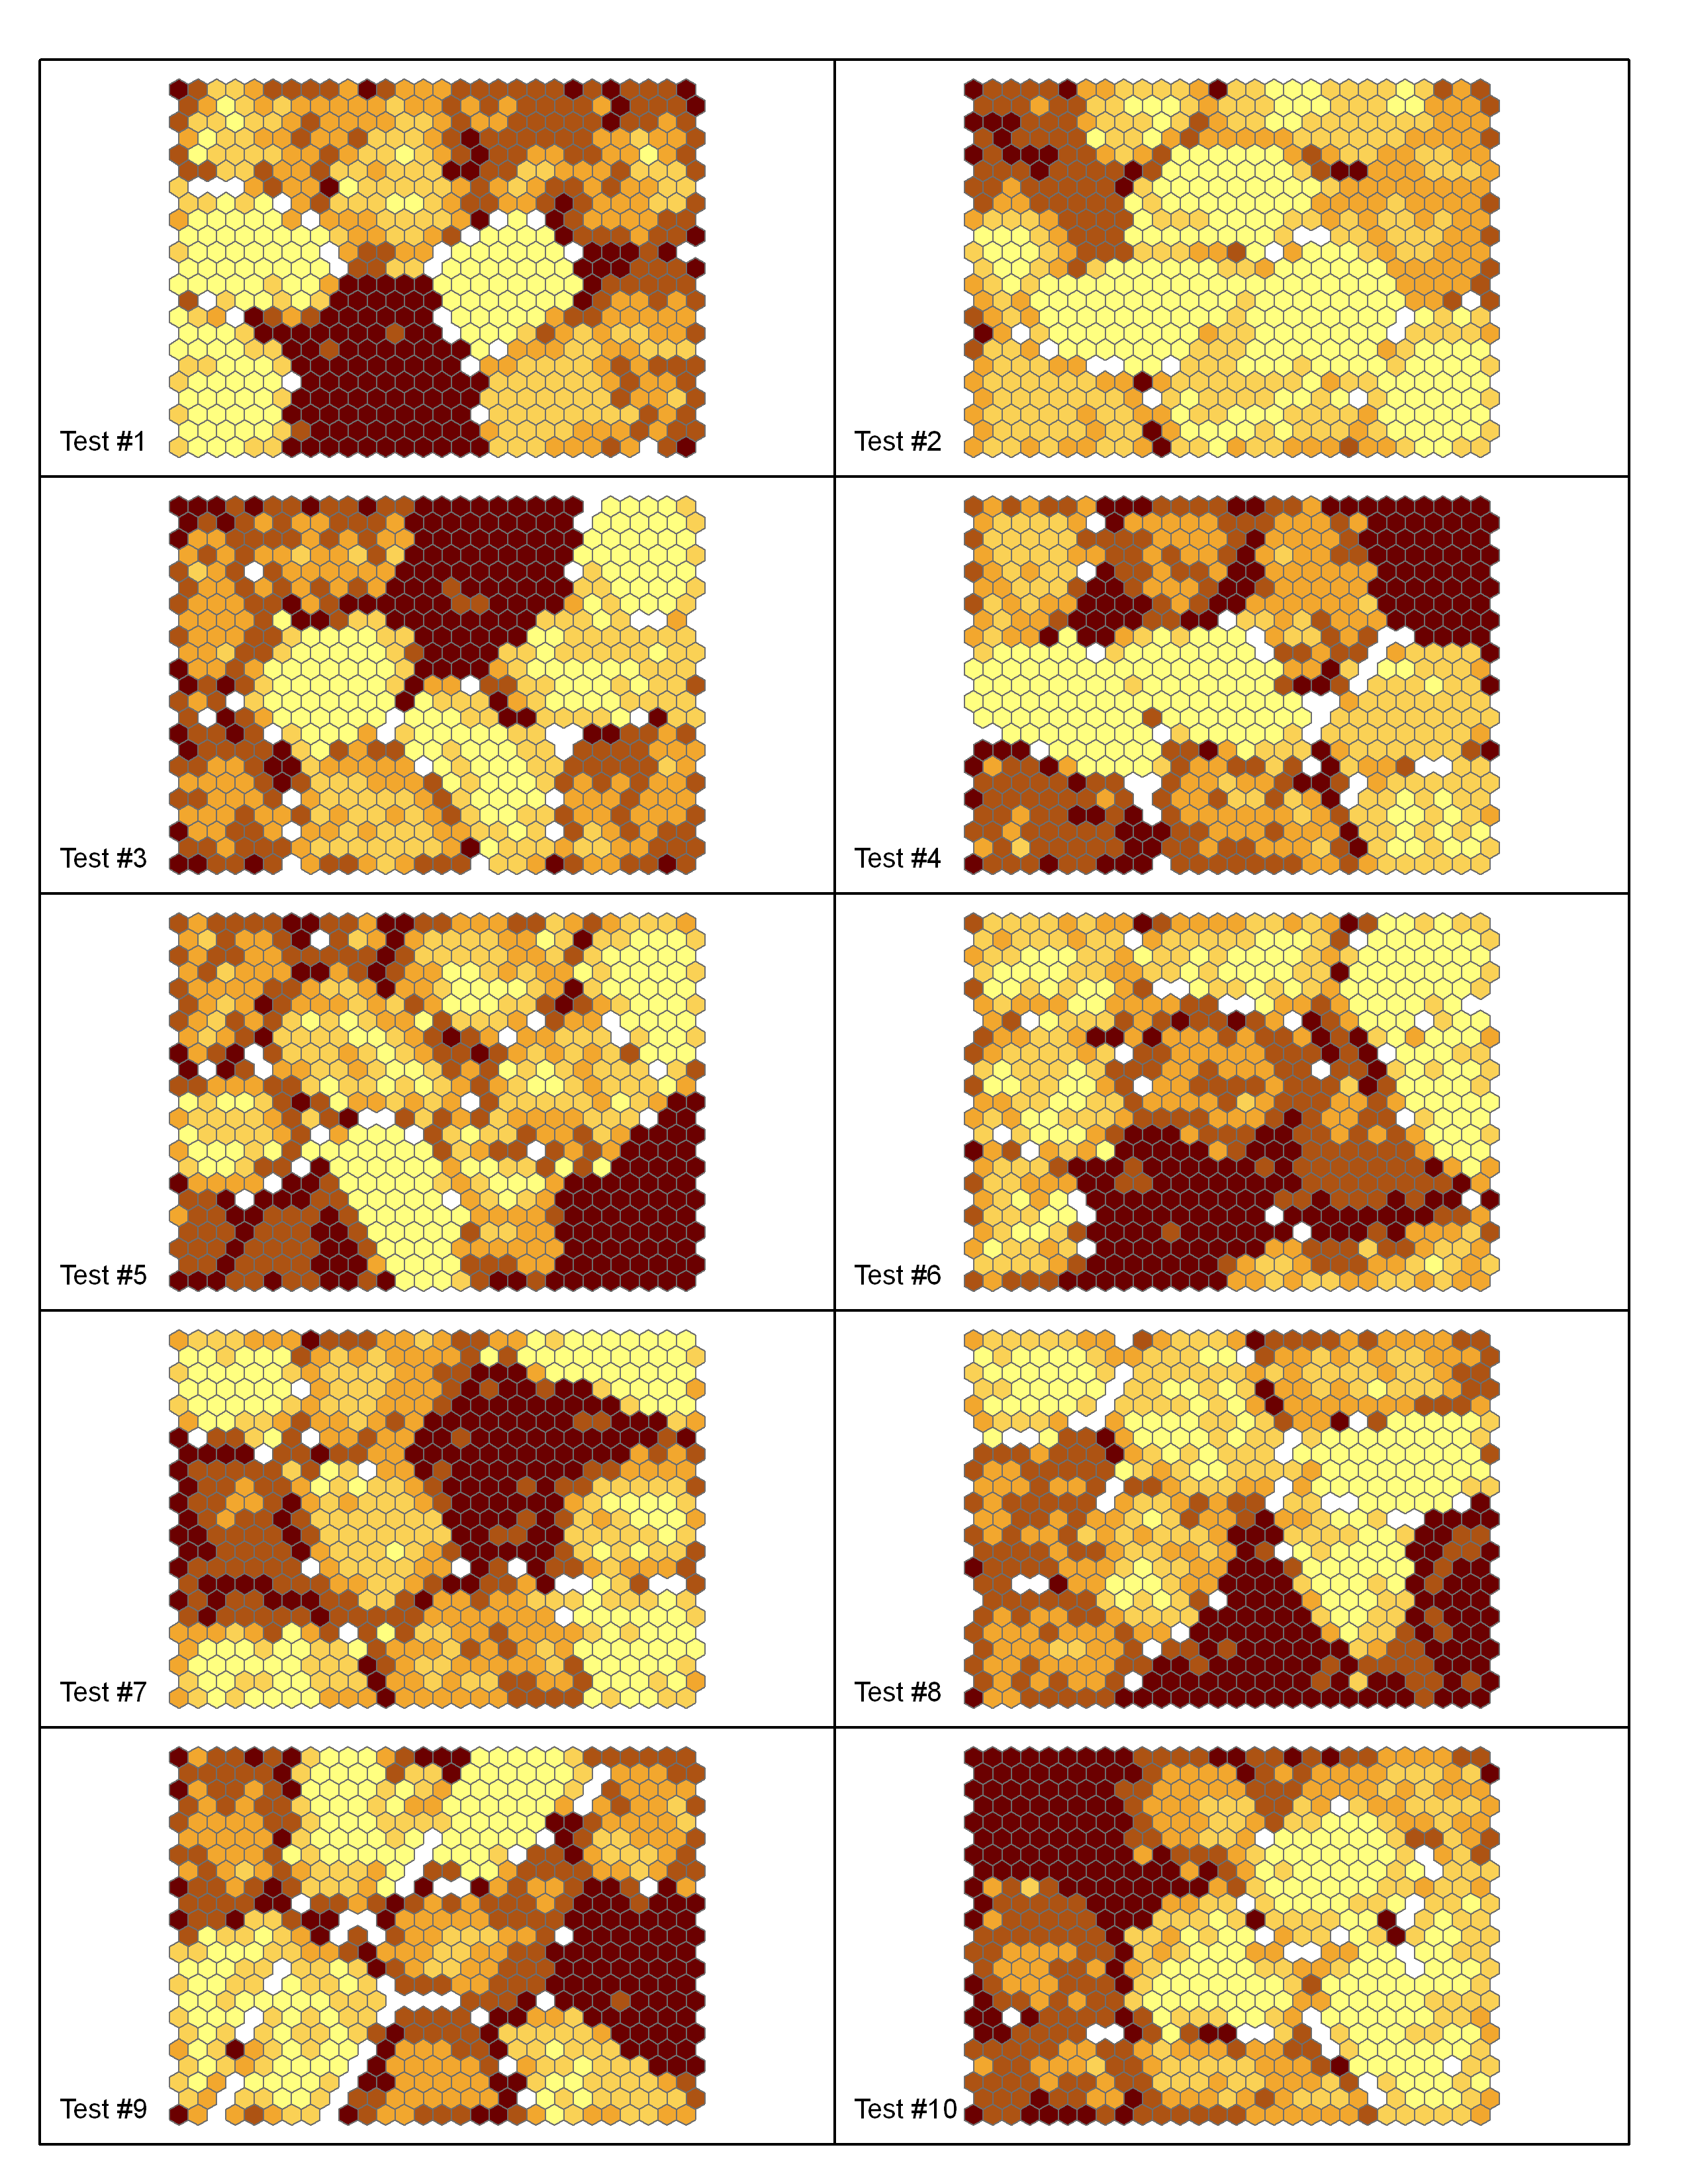
\includegraphics[width=.40\linewidth]{hex_10.png}
}
\subfigure[Spherical Topology]{
  \label{ten:graph}
  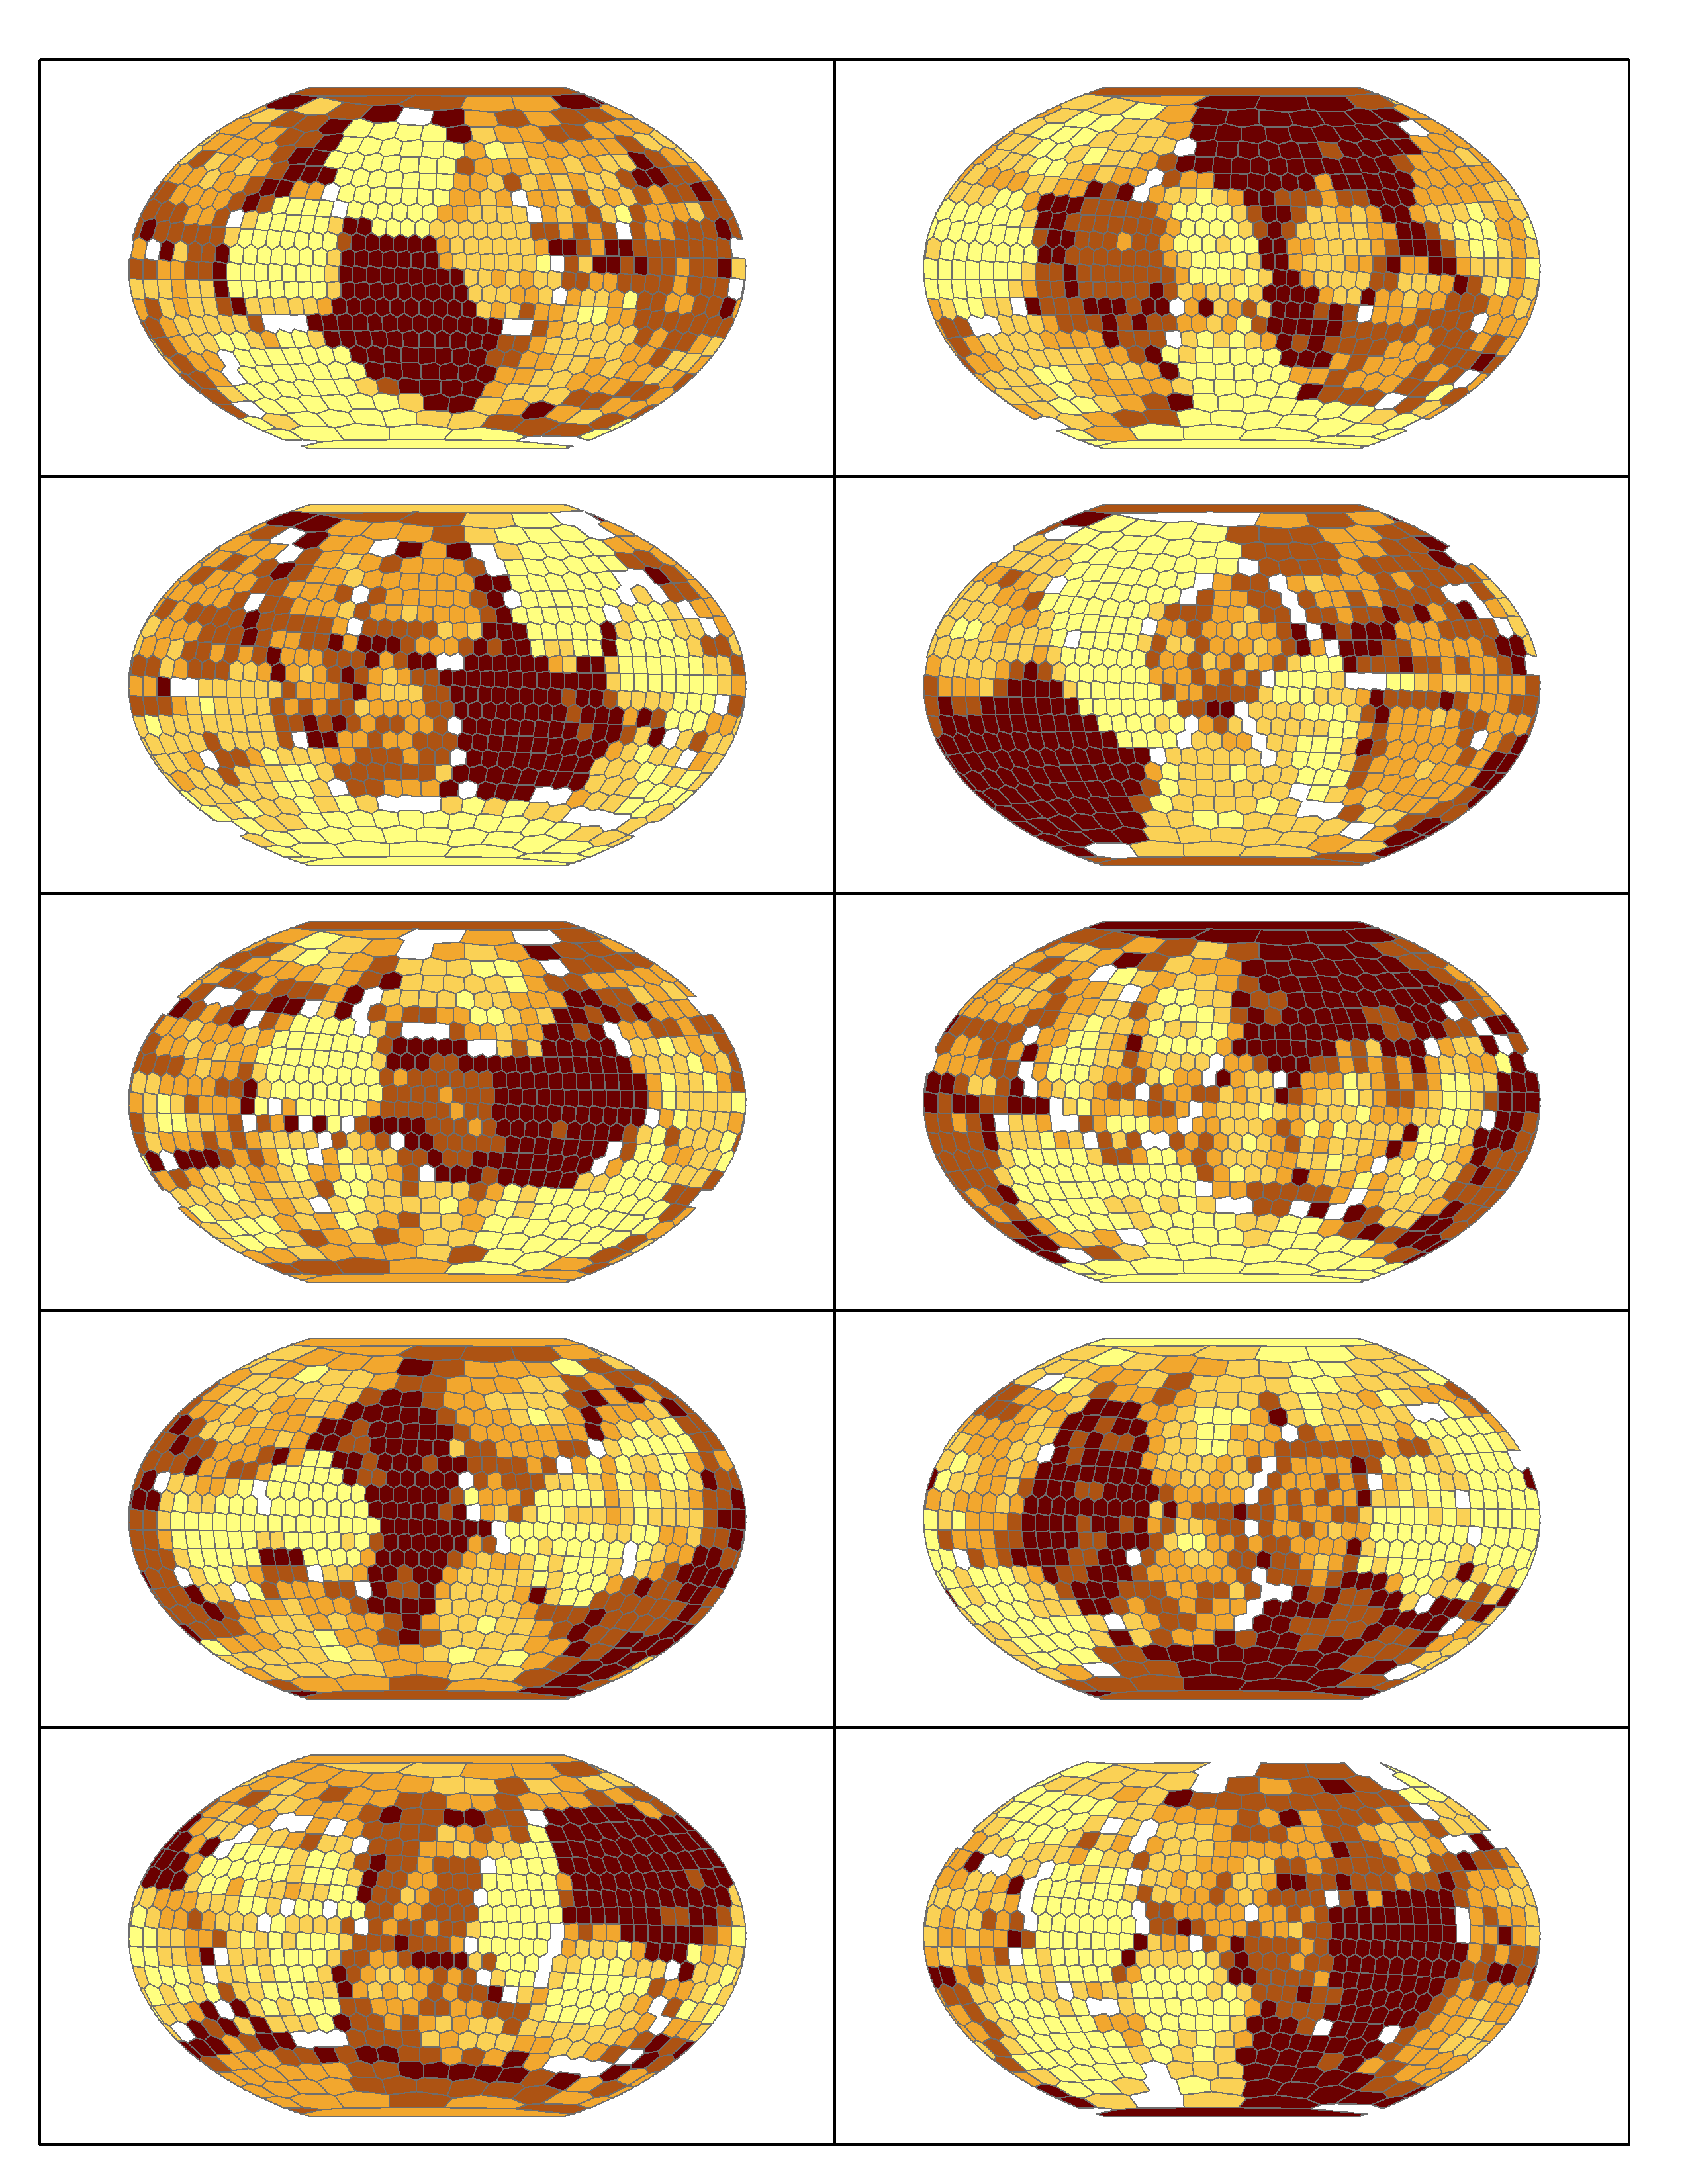
\includegraphics[width=.40\linewidth]{sphere_winkel.png}
}
\subfigure[Geodesic Sphere Topology]{
  \label{ten:geodesic}
  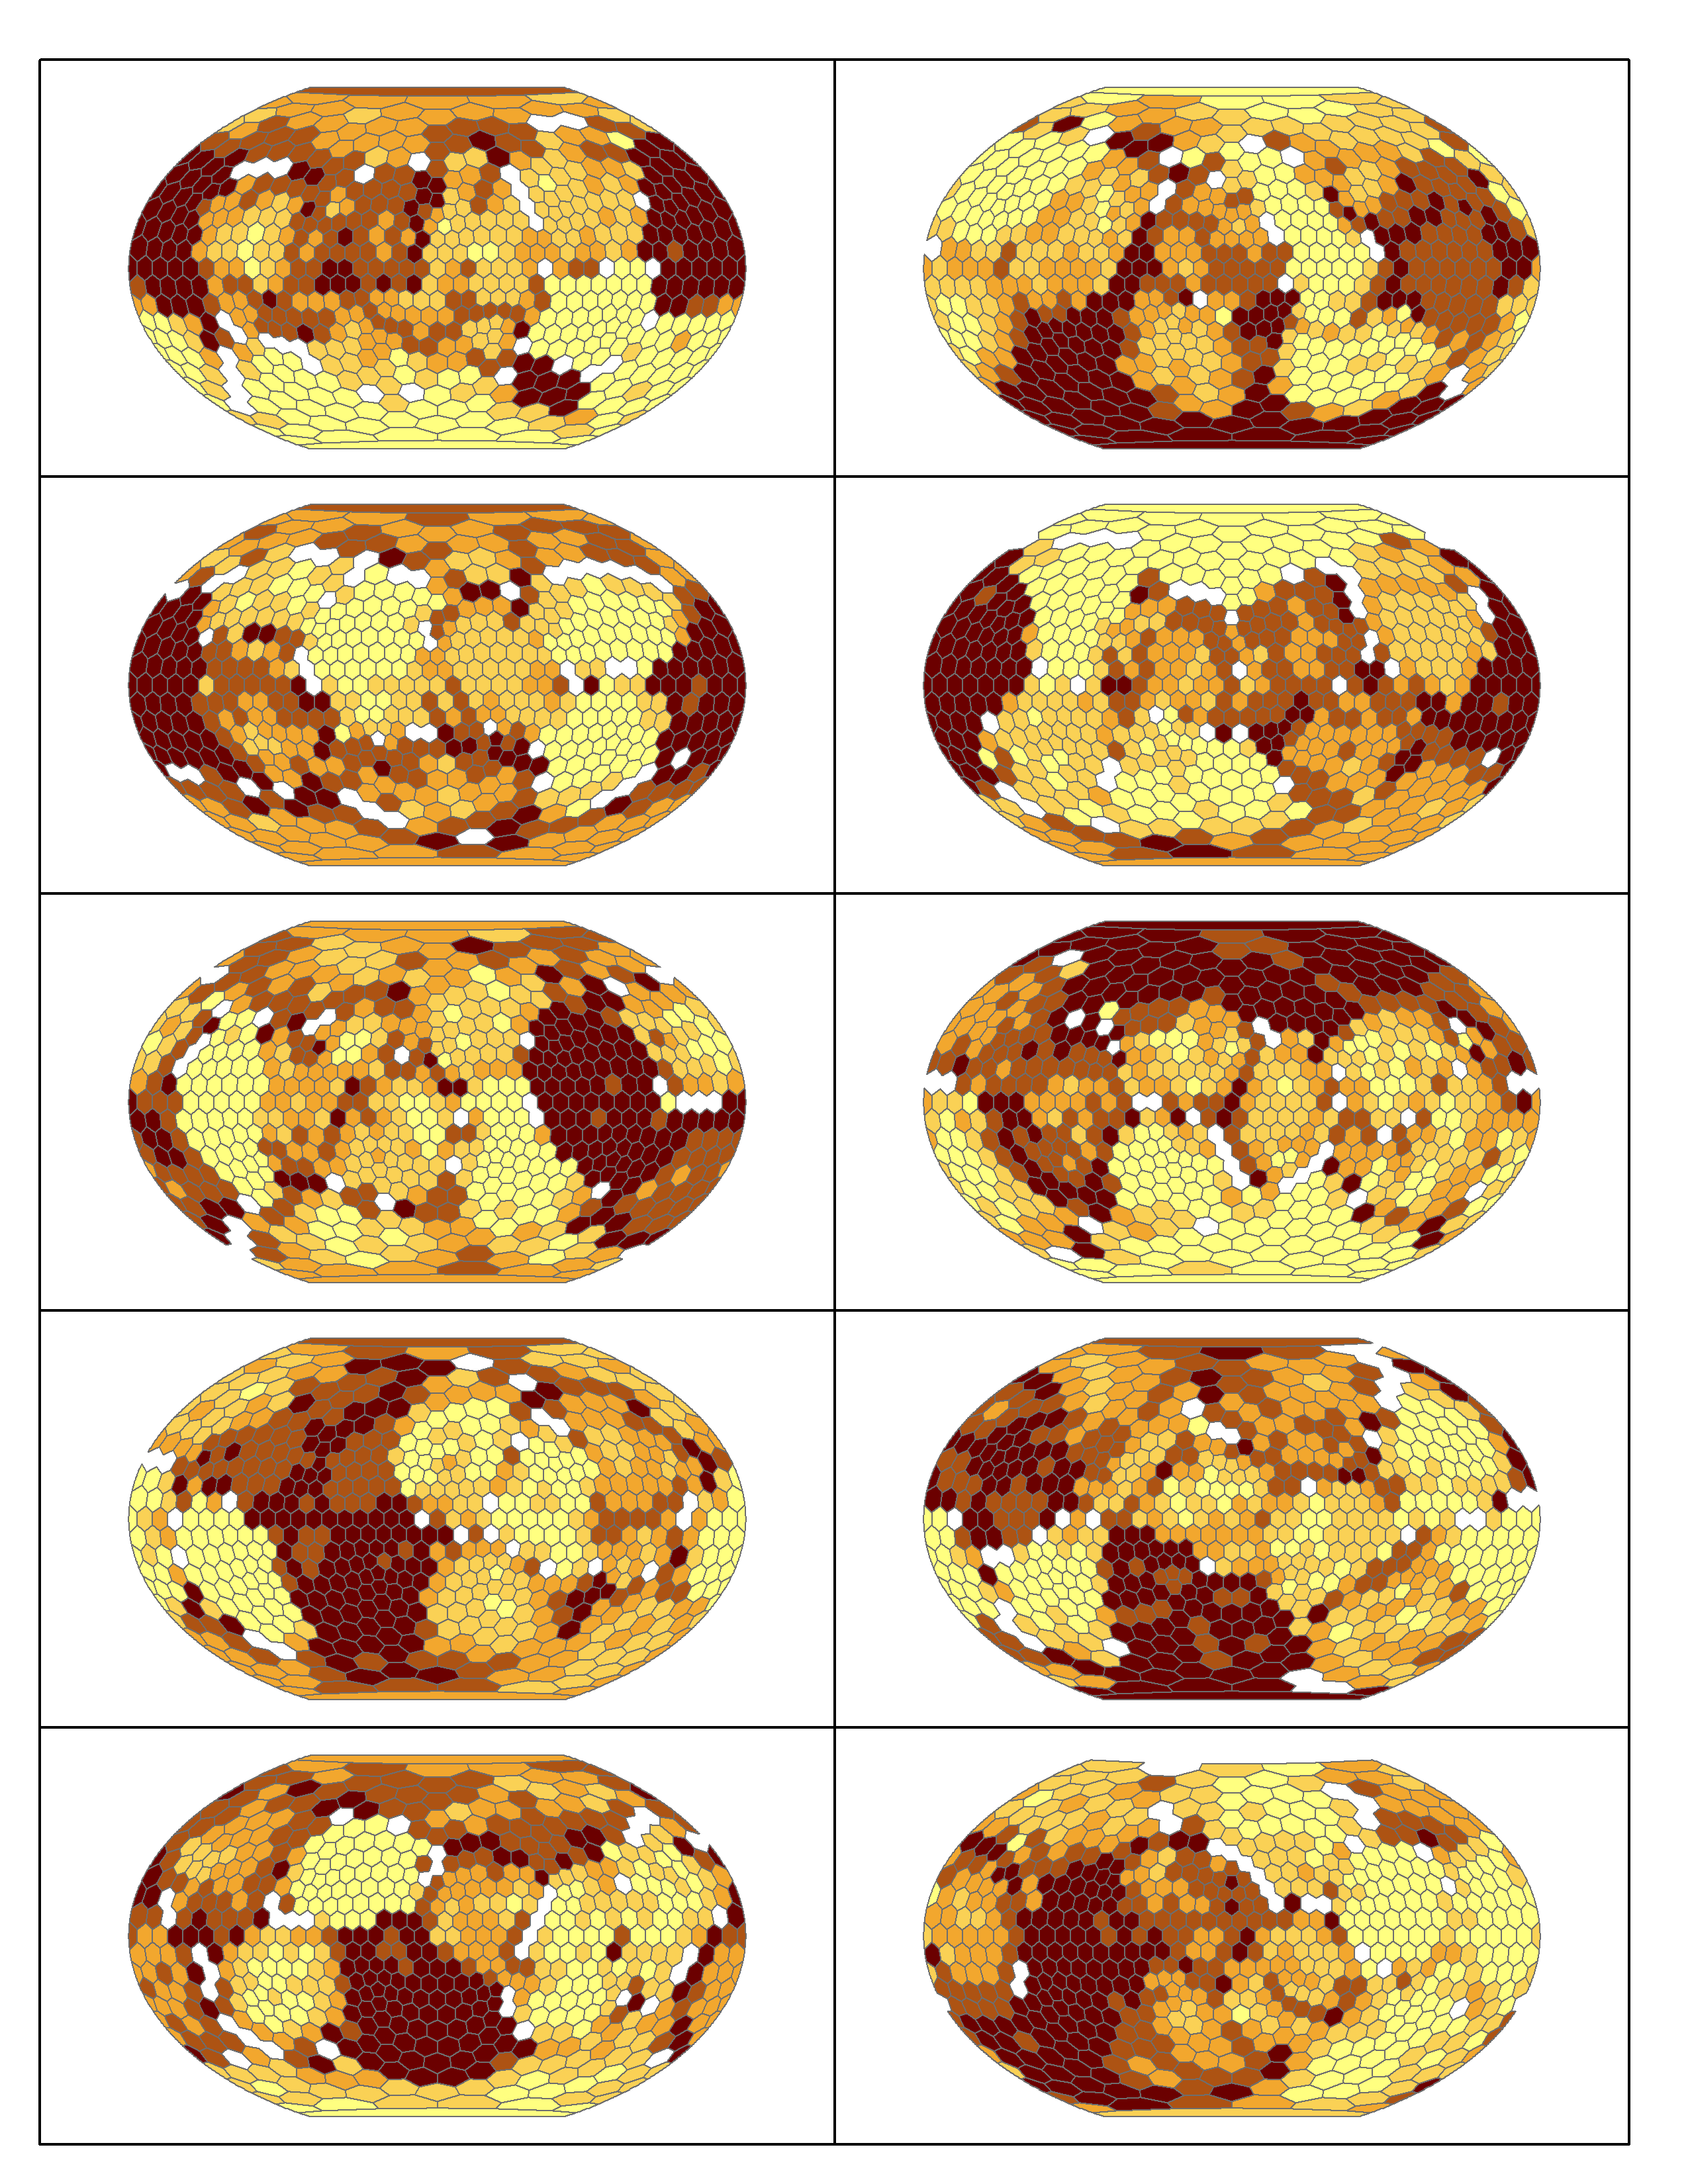
\includegraphics[width=.40\linewidth]{geodesic_winkel.png}
}
\caption{This shows 4 box plots, each representing one group of neurons in a set
of SOMs trained with the same parameters.}
\label{ten}
\end{figure}
